\section{Foundations of extended deformations of dimer models}\label{sec_proof}

In this section, we observe the fundamental properties of extended zig-deformations and zag-deformations.
In particular, we will pursue the change of zigzag paths under these deformations
in Sections~\ref{subsec_behave_zigzag} and~\ref{subsec_property_zigzag}.
We refer the reader to Appendix~\ref{app_large_example} for understanding those observation in a concrete example.

Throughout this section, we keep the notation of Sections~\ref{sec_def_deform} and~\ref{sec_def_exdeform} unless otherwise stated.

\subsection{The proof of the non-degeneracy}\label{subsec_nondegenerate_deformation}

In this subsection, we prove the non-degeneracy of the dimer models $\overline{\nu}^\zig_\calX(\Gamma, \{z_1,\dots,z_r\})$ and $\overline{\nu}^\zag_\calY(\Gamma, \{z_1,\dots,z_r\})$.

\begin{Proposition}\label{prop_nondegenerate}
The dimer models $\overline{\nu}^\zig_\calX(\Gamma, \{z_1,\dots,z_r\})$, and $\overline{\nu}^\zag_\calY(\Gamma, \{z_1,\dots,z_r\})$ are non-degenerate.
\end{Proposition}

\begin{proof}
We prove this for $\overline{\nu}^\zig_\calX(\Gamma)=\overline{\nu}^\zig_\calX(\Gamma, \{z_1,\dots,z_r\})$, the other case is similar.
Let $\Gamma^\prime$ be the dimer model obtained by applying the operations (zig-1)--(zig-3) to $\Gamma$.

{\it The first step.}
We recall that the non-degeneracy condition is equivalent to the strong marriage condition; that is, a dimer model has equal numbers of black and white nodes and every proper subset $S$ of the black nodes satisfies the condition that~$S$ is connected to at least $|S|+1$ white nodes.

Suppose that $\Gamma^\prime$ is non-degenerate. Then $\Gamma^\prime$ satisfies the strong marriage condition.
By applying the operation (zig-4), we obtain the dimer model $\overline{\nu}^\zig_\calX(\Gamma, \{z_1,\dots,z_r\})$.
Since (zig-4) is the operation that adds new edges, it also satisfies the strong marriage condition, and hence it is non-degenerate.
Therefore, it is enough to show that $\Gamma^\prime$ is non-degenerate.

{\it The second step.}
We next consider a sub-dimer motel $\Gamma^{\prime \prime}$ of $\Gamma$ satisfying the condition $(*)$ below.
Note that $\Gamma^{\prime\prime}$ is said to be a \emph{sub-dimer model} of $\Gamma$
if the set of the nodes coincide and the set of edges in $\Gamma^{\prime\prime}$ is a subset of edges in $\Gamma$.

Condition $(*)$: For any given edge $e$ in $\Gamma^{\prime\prime}$,
let $z'$ and $z''$ be the two different zigzag paths on~$\Gamma^{\prime\prime}$ containing $e$.
Then either $(*1)$ or $(*2)$ holds:
\begin{itemize}
\setlength{\parskip}{0pt}
\itemsep=0pt
\setlength{\leftskip}{0.3cm}
\item[$(*1)$] Either $[z'] \in \{[z_i],-[z_i]\}$ or $[z''] \in \{[z_i],-[z_i]\}$ holds;
\item[$(*2)$] For any $i$, if $z'$ intersects with $z_i$ in $\Zig(z_i)$ (resp.~$\Zag(z_i)$), then $z''$ intersects with $z_i$ in~$\Zag(z_i)$ (resp.~$\Zig(z_i)$).
\end{itemize}

A sub-dimer model $\Gamma^{\prime \prime}$ of $\Gamma$ satisfying $(*)$ can be constructed using
the algorithm developed in~\cite{Gul,IU2} for proving Theorem~\ref{existence_dimer}.
We adapt it to our situation.

First, let us consider the original dimer model $\Gamma$ and let $E_1,E_2,\dots,E_m$ be all edges of $\Delta_\Gamma$, where the primitive outer normal vector for $E_1$ is the slope $[z_1]=\cdots=[z_r]$.
We assume that these edges are ordered cyclically in the anti-clockwise direction (see Figure~\ref{PMpolygon_normalvec} as a reference).
Also, let $v_j$ be the primitive outer normal vector corresponding to~$E_j$, for $1 \leq j \leq m$.
Let~$a$ be the index such that $v_a=-v_1$ if there exists such an edge among $E_2,\dots,E_m$; that is, $E_a$~is parallel to~$E_1$.
If there is no such edge, then let $E_a= \varnothing$ for simplicity of notation.
We recall that by Proposition~\ref{zigzag_sidepolygon}, for each $E_j\neq\varnothing$ there exist zigzag paths on $\Gamma$ such that the associated slopes coincide with $v_j$, and the set of such zigzag paths is denoted by $\calZ_{v_j}=\calZ_{v_j}(\Gamma)$.
By our assumption, each slope of the zigzag paths in $\calZ_1\coloneqq\calZ_{v_2}\cup\cdots\cup\calZ_{v_{a-1}}$ and $v_1$ are linearly independent.
Thus, the zigzag paths in $\calZ_1$ intersect with a type~I zigzag path $z_i$ precisely once in the universal cover (see Lemma~\ref{slope_linearly_independent}).
By definition of $E_2,\dots,E_{a-1}$, such an intersection is given from the right of $z_i$ to the left of $z_i$,
and hence zigzag paths in $\calZ_1$ intersect with~$z_i$ in~$\Zag(z_i)$.
Similarly, we find that the zigzag paths in $\calZ_2\coloneqq\calZ_{v_{a+1}}\cup\cdots\cup\calZ_{v_m}$ intersect with $z_i$ precisely once in the universal cover, and specifically, they intersect with $z_i$ in $\Zig(z_i)$.

If there are at least two edges between $E_2$ and $E_{a-1}$ (i.e., $a \geq 4$),
then we take two adjacent edges, say, $E_2$ and~$E_3$.
Since $v_2$ and $v_3$ are linearly independent, the zigzag paths $z_2'\in\calZ_{v_2}$ and $z_3'\in\calZ_{v_3}$ intersect at some edge of $\Gamma$.
Clearly, such an intersection $z_2' \cap z_3'$ is neither any edge constituting any zigzag path whose slope is $[z_i]$ nor $-[z_i]$.
Now, remove an edge in $z_2' \cap z_3'$. This operation merges $z_2'$ and $z_3'$, in which case the resulting dimer model stays consistent and the associated PM polygon
changes into the polygon obtained by cutting the corner of the original PM polygon consisting of edges whose outer normal vectors are $[z_2']$ and $[z_3']$
(see \cite[Sections~5 and 6]{Gul} for more details).
Furthermore, since $z_2' \cap z_i \subset \Zag(z_i)$ and $z_3' \cap z_i \subset \Zag(z_i)$ for each~$i$, edges in $z_2' \cap z_3'$ do not share a node with $z_i$ for any $i$.
Thus, $z_i$ is still type I even if we apply this operation and the merged zigzag path intersects with $z_i$ in $\Zag(z_i)$ .
We repeat this procedure until there are no two edges between $E_2$ and $E_{a-1}$.

Similarly, if there are at least two edges between $E_{a+1}$ and $E_m$ (i.e., $m-a \geq 2$), then we do the same procedures as above until there are no two edges between~$E_{a+1}$ and~$E_m$.
After removing all suitable edges from $\Gamma$, we get a consistent dimer model, which is clearly a sub-dimer model of~$\Gamma$,
and we denote this by~$\Gamma_{\sf sub}$.
Since we do not remove edges contained in a zigzag path whose slope is~$\pm[z_i]$ in the above arguments,
the edges~$E_1$ and~$E_a$ (if this is not empty) of $\Delta_\Gamma$ are preserved on $\Delta_{\Gamma_{\sf sub}}$ (and hence we will use the same notation).
Also, the edges $E_2,\dots,E_{a-1}$ (resp.~$E_{a+1},\dots,E_m$) of $\Delta_\Gamma$ are substituted by a single edge in $\Delta_{\Gamma_{\sf sub}}$.
We denote such an edge by $E_2^\prime$ (resp.~$E_m^\prime$).
We note that zigzag paths corresponding to $E_2^\prime$ (resp.~$E_m^\prime$) are obtained by merging the ones corresponding to $E_2,\dots,E_{a-1}$ (resp.~$E_{a+1},\dots,E_m$).
In particular, the PM polygon $\Delta_{\Gamma_{\sf sub}}$ is formed by $E_1$, $E_2^\prime$, $E_a$, $E_m^\prime$, in which case $\Delta_{\Gamma_{\sf sub}}$ is a triangle or a trapezoid.
Then, it follows from the construction of $\Gamma_{\sf sub}$ that
\begin{itemize}\itemsep=0pt
\item[--] the zigzag paths $z_1,\dots,z_r$ on $\Gamma$ are preserved on $\Gamma_{\sf sub}$ and they are type~I;
\item[--] the zigzag paths on $\Gamma$ corresponding to $E_a$ (if this is not empty) are preserved on $\Gamma_{\sf sub}$;
\item[--] the zigzag paths corresponding to $E_2^\prime$ (resp.~$E_m^\prime$) are intersected with $z_i$ in $\Zag(z_i)$ (resp.\ $\Zig(z_i)$)
(see also the argument in the proof of Lemma~\ref{intersect_zigorzag}).
\end{itemize}
From these facts, it is easy to verify that $\Gamma_{\sf sub}$ is a sub-dimer model $\Gamma^{\prime\prime}$ of $\Gamma$ satisfying the condition $(*)$.

{\it The third step.}
Now, we apply the operations (zig-1)--(zig-3) in Definition \ref{def_deformation_zig} to $\Gamma_{\sf sub}$,
which is possible since $z_1,\dots,z_r$ are preserved on~$\Gamma_{\sf sub}$.
We denote the resulting dimer model by~$\Gamma^\prime_{\sf sub}$.
By construction, $\Gamma^\prime$ can be obtained by adding some edges to $\Gamma^\prime_{\sf sub}$. Thus, similar to the discussion in the first step, it is enough to show that $\Gamma^\prime_{\sf sub}$ is non-degenerate to prove the non-degeneracy of~$\Gamma^\prime$.

Thus, we now show that $\Gamma^\prime_{\sf sub}$ is non-degenerate.
To do this, we prove the existence of a~perfect matching that contains a given edge $e$ of $\Gamma^\prime_{\sf sub}$.
We divide the set of edges into four cases~(i)--(iv):
\begin{itemize}\itemsep=0pt
\item[(i)] $e$ is of the form $(b_{i,j-1}[2m-1], w_{i,j}[2m-1])$ for some $1 \leq i \leq r, 1 \leq j \leq p_i+1$ and $1 \leq m \leq n$,
where we let $b_{i,0}[2m-1]=b_i[2m-1]$ and $w_{i,p_i+1}[2m-1]=w_i[2m-1]$;
\item[(ii)] $e$ is of the form $(w_{i,j}[2m-1], b_{i,j}[2m-1])$ for some $1 \leq i \leq r, 1 \leq j \leq p_i$ and $1 \leq m \leq n$;
\item[(iii)] $e$ is of the form $(b_{i,j}[2m-1],w_{i,j}[2m-3])$ for some $1 \leq i \leq r, 1 \leq j \leq p_i$ and $1 \leq m \leq n$;
\item[(iv)] $e$ is of a form other than those in (i)--(iii).
\end{itemize}
Namely, (i) and (ii) are the edges emanating from the process (zig-1), (iii) is an edge added in the process (zig-3), and (iv) is an edge that is invariant between $\Gamma^\prime_{\sf sub}$ and $\Gamma_{\sf sub}$.

Since $\Gamma_{\sf sub}$ is consistent and contains the type I zigzag paths $z_1,\dots,z_r$,
there exist corner perfect matchings $\sfP$ and $\sfP^\prime$ on $\Gamma_{\sf sub}$ that are adjacent and satisfy $\sfP \cap z_i=\Zig(z_i)$ and $\sfP^\prime \cap z_i=\Zag(z_i)$ for $1 \leq i \leq r$ (see Section~\ref{subsec_relation_zigzag_pm}).
Similarly, let~$\sfQ$ be a corner perfect matching on $\Gamma_{\sf sub}$ with $\sfQ \cap z_i = \varnothing$ for $1 \leq i \leq r$.
The existence of such~$\sfQ$ is guaranteed by Lemma~\ref{lem_existence_pm}.
We will use these $\sfP$, $\sfP^\prime$ and $\sfQ$ in order to find a suitable perfect matching on $\Gamma^\prime_{\sf sub}$ containing a given edge $e$.
We divide our discussions into the following cases (i)--(iv) that correspond to the above division of edges.

Case (i): Let \begin{gather}\label{PM_case(i)}
\sfP^{\prime\prime}=\bigg(\sfP \setminus \bigcup_{i=1}^r \Zig(z_i)\bigg) \cup \bigg(\bigcup_{i=1}^r \bigcup_{j=1}^{p_i+1} \bigcup_{m=1}^n(b_{i,j-1}[2m-1],w_{i,j}[2m-1])\bigg);
\end{gather}
see Figure~\ref{deformation_PM_i}. It is easy to see that $\sfP^{\prime\prime}$ is a perfect matching on $\Gamma^\prime_{\sf sub}$ containing $e$ in the case~(i).

Case (ii): Let \begin{gather*}%\label{PM_case(ii)}
\sfP^{\prime\prime}=\sfQ \cup \bigg(\bigcup_{i=1}^r \bigcup_{j=1}^{p_i} \bigcup_{m=1}^n(w_{i,j}[2m-1],b_{i,j}[2m-1])\bigg);
\end{gather*}
see Figure~\ref{deformation_PM_ii}. Then, we see that $\sfP^{\prime\prime}$ is a perfect matching on $\Gamma^\prime_{\sf sub}$ containing $e$ in the case~(ii).

Case (iii): Let \begin{displaymath}
\sfP^{\prime\prime}=\sfQ \cup \bigg(\bigcup_{i=1}^r \bigcup_{j=1}^{p_i} \bigcup_{m=1}^n(b_{i,j}[2m-1],w_{i,j}[2m-3])\bigg); \end{displaymath}
see Figure~\ref{deformation_PM_iii}. Then, we see that $\sfP^{\prime\prime}$ is a perfect matching on $\Gamma^\prime_{\sf sub}$ containing~$e$ in the case~(iii).

Case (iv): We note that an edge $e$ in the case (iv) also appears in $\Gamma_{\sf sub}$, since~$e$ is unchanged even if we apply (zig-1)--(zig-3).
Thus, we can regard $e$ as an edge of $\Gamma_{\sf sub}$.
Since $\Gamma_{\sf sub}$ satisfies the condition $(*)$, the zigzag paths $z^\prime$, $z^{\prime\prime}$ on~$\Gamma_{\sf sub}$ that contain $e$ satisfy
either $(*1)$ or $(*2)$.
\begin{itemize}\itemsep=0pt
\item We assume that $z^\prime$ and $z^{\prime\prime}$ satisfy $(*1)$.
\begin{itemize}\itemsep=0pt
\item Let, say, $[z^\prime]=[z_i]$.
Since zigzag paths having the same slopes are obtained as the difference of adjacent corner perfect matchings, either $\sfP$ or $\sfP^\prime$ contains $e$.
If $e \in \sfP$, then we let $\sfP^{\prime\prime}$ be as in~\eqref{PM_case(i)}.
Then, $\sfP^{\prime\prime}$ is a perfect matching on $\Gamma^\prime_{\sf sub}$ containing $e$.
Even if $e \in \sfP^\prime$, we have the same conclusion by letting
\begin{displaymath}
\sfP^{\prime\prime}=\bigg(\sfP^\prime \setminus \bigcup_{i=1}^r \Zag(z_i)\bigg) \cup \bigg(\bigcup_{i=1}^r \bigcup_{j=1}^{p_i+1} \bigcup_{m=1}^n(b_{i,j-1}[2m-1],w_{i,j}[2m-1])\bigg).
\end{displaymath}
\item Let, say, $[z^\prime]=-[z_i]$, in which case $E_a\neq \varnothing$ and $z^\prime$ corresponds to~$E_a$.
Let $\sfQ^\prime$ and $\sfQ^{\prime\prime}$ be the corner perfect matchings on~$\Gamma_{\sf sub}$ whose difference forms $z'$. Let $e \in \sfQ^\prime$.
Since $h(\sfQ^\prime,\sfP_0)$ lies on $E_a$, where $\sfP_0$ is the reference perfect matching, we have $\sfQ^\prime\cap z_i=\varnothing$ for any $i$ by Lemma~\ref{zigzag_lem1}.
Thus, we let
\begin{displaymath}
\sfP^{\prime\prime}=\sfQ^\prime \cup \bigg(\bigcup_{i=1}^r \bigcup_{j=1}^{p_i} \bigcup_{m=1}^n(w_{i,j}[2m-1],b_{i,j}[2m-1])\bigg),
\end{displaymath}
and see that $\sfP^{\prime\prime}$ is a perfect matching on $\Gamma^\prime_{\sf sub}$ containing $e$.
\end{itemize}
\item We assume that $z^\prime$ and $z^{\prime\prime}$ satisfy $(*2)$.

Let, say, $z'$ intersect with each $z_i$ in $\Zig(z_i)$. Let $\sfQ^\prime$ and $\sfQ^{\prime\prime}$ be the corner perfect matchings on $\Gamma_{\sf sub}$ whose difference forms $z'$. Let $e \in \sfQ^\prime$.
As noted above, we see that all zigzag paths in $\Gamma_{\sf sub}$ intersecting with $z_i$ at some zig of $z_i$ have the same slopes.
This implies that $\sfQ^\prime$ contains all zigs of~$z_i$, i.e., $\sfQ^\prime \cap z_i=\Zig(z_i)$. This also means that $\sfQ^\prime=\sfP$.
Hence, we let~$\sfP^{\prime\prime}$ be the same as~\eqref{PM_case(i)} and see that $\sfP^{\prime\prime}$ is a perfect matching containing~$e$.\hfill\qed
\end{itemize}
\renewcommand{\qed}{}
\end{proof}

\begin{figure}[h!]\centering\vspace*{-10mm}
\scalebox{0.55}{
\begin{tikzpicture}
\newcommand{\edgewidth}{0.05cm} %line_width_of _edges
\newcommand{\nodewidth}{0.05cm} %line_width_around_nodes
\newcommand{\noderad}{0.16} %radius_of_node

\newcommand{\pmwidth}{0.35cm}
\newcommand{\pmcolor}{red}

%coordinate setting
\coordinate (W1) at (0,1.2); \coordinate (W2) at (0,3.6);
%\coordinate (B1) at (3,0); \coordinate (B2) at (3,2.4);
\path (W1) ++(-20:4cm) coordinate (B1); \path (W2) ++(-20:4cm) coordinate (B2);
\path (B1) ++(200:2cm) coordinate (B0); \path (W2) ++(20:2cm) coordinate (W3);

\path (W1) ++(-20:0.8cm) coordinate (B1-1); \path (W1) ++(-20:1.6cm) coordinate (W1-1);
\path (W1) ++(-20:2.4cm) coordinate (B1-2); \path (W1) ++(-20:3.2cm) coordinate (W1-2);
\path (W2) ++(-20:0.8cm) coordinate (B2-1); \path (W2) ++(-20:1.6cm) coordinate (W2-1);
\path (W2) ++(-20:2.4cm) coordinate (B2-2); \path (W2) ++(-20:3.2cm) coordinate (W2-2);

\path (B1) ++(40:1cm) coordinate (B1e); \path (B1) ++(320:1cm) coordinate (B1s); \path (B1) ++(20:0.9cm) coordinate (B1es);
\path (W1) ++(140:1cm) coordinate (W1w); \path (W1) ++(220:1cm) coordinate (W1s); \path (W1) ++(200:0.9cm) coordinate (W1ws);
\path (B2) ++(40:1cm) coordinate (B2e); \path (B2) ++(320:1cm) coordinate (B2s); \path (B2) ++(20:0.9cm) coordinate (B2es);
\path (W2) ++(140:1cm) coordinate (W2w); \path (W2) ++(220:1cm) coordinate (W2s); \path (W2) ++(200:0.9cm) coordinate (W2ws);

\path (W1) ++(150:0.7cm) coordinate (W1+); \path (W2) ++(150:0.7cm) coordinate (W2+);
\path (B1) ++(330:0.7cm) coordinate (B1-); \path (B2) ++(330:0.7cm) coordinate (B2-);

\node (original) at (0,0) {
\begin{tikzpicture}
%perfect matching
\draw [\pmcolor, line width=\pmwidth] (B1)--(W1);
\draw [\pmcolor, line width=\pmwidth] (B2)--(W2);
%edge
\draw [line width=\edgewidth] (B1)--(W1); \draw [line width=\edgewidth] (B2)--(W1) ; \draw [line width=\edgewidth] (B2)--(W2) ;
\draw [line width=\edgewidth] (B1)--(B0) ; \draw [line width=\edgewidth] (W2)--(W3) ;
\draw [line width=\edgewidth] (B1)--(B1e); \draw [line width=\edgewidth] (B1)--(B1s); \draw [line width=\edgewidth] (B1)--(B1es);
\draw [line width=\edgewidth] (W1)--(W1w); \draw [line width=\edgewidth] (W1)--(W1s); \draw [line width=\edgewidth] (W1)--(W1ws);
\draw [line width=\edgewidth] (B2)--(B2e); \draw [line width=\edgewidth] (B2)--(B2s); \draw [line width=\edgewidth] (B2)--(B2es);
\draw [line width=\edgewidth] (W2)--(W2w); \draw [line width=\edgewidth] (W2)--(W2s); \draw [line width=\edgewidth] (W2)--(W2ws);

\draw [line width=\edgewidth,line cap=round, dash pattern=on 0pt off 2.5\pgflinewidth] (W1+)-- ++(-90:0.5cm);
\draw [line width=\edgewidth,line cap=round, dash pattern=on 0pt off 2.5\pgflinewidth] (W2+)-- ++(-90:0.5cm);
\draw [line width=\edgewidth,line cap=round, dash pattern=on 0pt off 2.5\pgflinewidth] (B1-)-- ++(90:0.5cm);
\draw [line width=\edgewidth,line cap=round, dash pattern=on 0pt off 2.5\pgflinewidth] (B2-)-- ++(90:0.5cm);

%blacknode
\draw [line width=\nodewidth, fill=black] (B1) circle [radius=\noderad] ; \draw [line width=\nodewidth, fill=black] (B2) circle [radius=\noderad] ;
%whitenode
\draw [line width=\nodewidth, fill=white] (W1) circle [radius=\noderad] ; \draw [line width=\nodewidth, fill=white] (W2) circle [radius=\noderad] ;

\end{tikzpicture}};


\node (predeformed) at (12,0) {
\begin{tikzpicture}
\path (B1-1) ++(-70:1.5cm) coordinate (B1-1-); \path (B1-2) ++(-70:1.5cm) coordinate (B1-2-);
\path (W2-1) ++(110:1.5cm) coordinate (W2-1-); \path (W2-2) ++(110:1.5cm) coordinate (W2-2-);

%perfect matching
\draw [\pmcolor, line width=\pmwidth] (W1)--(B1-1); \draw [\pmcolor, line width=\pmwidth] (W1-1)--(B1-2); \draw [\pmcolor, line width=\pmwidth] (W1-2)--(B1);
\draw [\pmcolor, line width=\pmwidth] (W2)--(B2-1); \draw [\pmcolor, line width=\pmwidth] (W2-1)--(B2-2); \draw [\pmcolor, line width=\pmwidth] (W2-2)--(B2);
%edge
\draw [line width=\edgewidth] (B1)--(W1); \draw [line width=\edgewidth] (B2)--(W2) ;
\draw [line width=\edgewidth] (B1)--(B1e); \draw [line width=\edgewidth] (B1)--(B1s); \draw [line width=\edgewidth] (B1)--(B1es);
\draw [line width=\edgewidth] (W1)--(W1w); \draw [line width=\edgewidth] (W1)--(W1s); \draw [line width=\edgewidth] (W1)--(W1ws);
\draw [line width=\edgewidth] (B2)--(B2e); \draw [line width=\edgewidth] (B2)--(B2s); \draw [line width=\edgewidth] (B2)--(B2es);
\draw [line width=\edgewidth] (W2)--(W2w); \draw [line width=\edgewidth] (W2)--(W2s); \draw [line width=\edgewidth] (W2)--(W2ws);

\draw [line width=\edgewidth,line cap=round, dash pattern=on 0pt off 2.5\pgflinewidth] (W1+)-- ++(-90:0.5cm);
\draw [line width=\edgewidth,line cap=round, dash pattern=on 0pt off 2.5\pgflinewidth] (W2+)-- ++(-90:0.5cm);
\draw [line width=\edgewidth,line cap=round, dash pattern=on 0pt off 2.5\pgflinewidth] (B1-)-- ++(90:0.5cm);
\draw [line width=\edgewidth,line cap=round, dash pattern=on 0pt off 2.5\pgflinewidth] (B2-)-- ++(90:0.5cm);

\draw [line width=\edgewidth] (B2-1)--(W1-1); \draw [line width=\edgewidth] (B2-2)--(W1-2);
\draw [line width=\edgewidth] (B1-1)--(B1-1-); \draw [line width=\edgewidth] (B1-2)--(B1-2-);
\draw [line width=\edgewidth] (W2-1)--(W2-1-); \draw [line width=\edgewidth] (W2-2)--(W2-2-);

%blacknode
\draw [line width=\nodewidth, fill=black] (B1) circle [radius=\noderad] ; \draw [line width=\nodewidth, fill=black] (B2) circle [radius=\noderad] ;
\draw [line width=\nodewidth, fill=black] (B1-1) circle [radius=\noderad] ; \draw [line width=\nodewidth, fill=black] (B1-2) circle [radius=\noderad] ;
\draw [line width=\nodewidth, fill=black] (B2-1) circle [radius=\noderad] ; \draw [line width=\nodewidth, fill=black] (B2-2) circle [radius=\noderad] ;
%whitenode
\draw [line width=\nodewidth, fill=white] (W1) circle [radius=\noderad] ; \draw [line width=\nodewidth, fill=white] (W2) circle [radius=\noderad] ;
\draw [line width=\nodewidth, fill=white] (W1-1) circle [radius=\noderad] ; \draw [line width=\nodewidth, fill=white] (W1-2) circle [radius=\noderad] ;
\draw [line width=\nodewidth, fill=white] (W2-1) circle [radius=\noderad] ; \draw [line width=\nodewidth, fill=white] (W2-2) circle [radius=\noderad] ;
\end{tikzpicture}};


\path (original) ++(0:4cm) coordinate (original+); \path (predeformed) ++(180:4cm) coordinate (predeformed+);
\draw [->, line width=\edgewidth] (original+)--(predeformed+) node[midway,xshift=0cm,yshift=0.5cm] {\Large (zig-1)--(zig-3)} ;

\end{tikzpicture}
}
\caption{The perfect matchings $\sfP$ on $\Gamma_{\sf sub}$ (left) and $\sfP^{\prime\prime}$ on $\Gamma^\prime_{\sf sub}$ (right) for the case (i).}
\label{deformation_PM_i}
\end{figure}

\begin{figure}[h!]\centering
\scalebox{0.55}{
\begin{tikzpicture}
\newcommand{\edgewidth}{0.05cm} %line_width_of _edges
\newcommand{\nodewidth}{0.05cm} %line_width_around_nodes
\newcommand{\noderad}{0.16} %radius_of_node

\newcommand{\pmwidth}{0.35cm}
\newcommand{\pmcolor}{red}

\node (original) at (0,0) {
\begin{tikzpicture}
%perfect matching
\draw [\pmcolor, line width=\pmwidth] (B1)--(B1es); \draw [\pmcolor, line width=\pmwidth] (B2)--(B2es);
\draw [\pmcolor, line width=\pmwidth] (W1)--(W1ws); \draw [\pmcolor, line width=\pmwidth] (W2)--(W2ws);
%edge
\draw [line width=\edgewidth] (B1)--(W1); \draw [line width=\edgewidth] (B2)--(W1) ; \draw [line width=\edgewidth] (B2)--(W2) ;
\draw [line width=\edgewidth] (B1)--(B0) ; \draw [line width=\edgewidth] (W2)--(W3) ;
\draw [line width=\edgewidth] (B1)--(B1e); \draw [line width=\edgewidth] (B1)--(B1s); \draw [line width=\edgewidth] (B1)--(B1es);
\draw [line width=\edgewidth] (W1)--(W1w); \draw [line width=\edgewidth] (W1)--(W1s); \draw [line width=\edgewidth] (W1)--(W1ws);
\draw [line width=\edgewidth] (B2)--(B2e); \draw [line width=\edgewidth] (B2)--(B2s); \draw [line width=\edgewidth] (B2)--(B2es);
\draw [line width=\edgewidth] (W2)--(W2w); \draw [line width=\edgewidth] (W2)--(W2s); \draw [line width=\edgewidth] (W2)--(W2ws);

\draw [line width=\edgewidth,line cap=round, dash pattern=on 0pt off 2.5\pgflinewidth] (W1+)-- ++(-90:0.5cm);
\draw [line width=\edgewidth,line cap=round, dash pattern=on 0pt off 2.5\pgflinewidth] (W2+)-- ++(-90:0.5cm);
\draw [line width=\edgewidth,line cap=round, dash pattern=on 0pt off 2.5\pgflinewidth] (B1-)-- ++(90:0.5cm);
\draw [line width=\edgewidth,line cap=round, dash pattern=on 0pt off 2.5\pgflinewidth] (B2-)-- ++(90:0.5cm);

%blacknode
\draw [line width=\nodewidth, fill=black] (B1) circle [radius=\noderad] ; \draw [line width=\nodewidth, fill=black] (B2) circle [radius=\noderad] ;
%whitenode
\draw [line width=\nodewidth, fill=white] (W1) circle [radius=\noderad] ; \draw [line width=\nodewidth, fill=white] (W2) circle [radius=\noderad] ;
\end{tikzpicture}};

\node (predeformed) at (12,0) {
\begin{tikzpicture}
\path (B1-1) ++(-70:1.5cm) coordinate (B1-1-); \path (B1-2) ++(-70:1.5cm) coordinate (B1-2-);
\path (W2-1) ++(110:1.5cm) coordinate (W2-1-); \path (W2-2) ++(110:1.5cm) coordinate (W2-2-);

%perfect matching
\draw [\pmcolor, line width=\pmwidth] (B1)--(B1es); \draw [\pmcolor, line width=\pmwidth] (B2)--(B2es);
\draw [\pmcolor, line width=\pmwidth] (W1)--(W1ws); \draw [\pmcolor, line width=\pmwidth] (W2)--(W2ws);
\draw [\pmcolor, line width=\pmwidth] (W1-1)--(B1-1); \draw [\pmcolor, line width=\pmwidth] (W1-2)--(B1-2);
\draw [\pmcolor, line width=\pmwidth] (W2-1)--(B2-1); \draw [\pmcolor, line width=\pmwidth] (W2-2)--(B2-2);
%edge
\draw [line width=\edgewidth] (B1)--(W1); \draw [line width=\edgewidth] (B2)--(W2) ;
\draw [line width=\edgewidth] (B1)--(B1e); \draw [line width=\edgewidth] (B1)--(B1s); \draw [line width=\edgewidth] (B1)--(B1es);
\draw [line width=\edgewidth] (W1)--(W1w); \draw [line width=\edgewidth] (W1)--(W1s); \draw [line width=\edgewidth] (W1)--(W1ws);
\draw [line width=\edgewidth] (B2)--(B2e); \draw [line width=\edgewidth] (B2)--(B2s); \draw [line width=\edgewidth] (B2)--(B2es);
\draw [line width=\edgewidth] (W2)--(W2w); \draw [line width=\edgewidth] (W2)--(W2s); \draw [line width=\edgewidth] (W2)--(W2ws);

\draw [line width=\edgewidth,line cap=round, dash pattern=on 0pt off 2.5\pgflinewidth] (W1+)-- ++(-90:0.5cm);
\draw [line width=\edgewidth,line cap=round, dash pattern=on 0pt off 2.5\pgflinewidth] (W2+)-- ++(-90:0.5cm);
\draw [line width=\edgewidth,line cap=round, dash pattern=on 0pt off 2.5\pgflinewidth] (B1-)-- ++(90:0.5cm);
\draw [line width=\edgewidth,line cap=round, dash pattern=on 0pt off 2.5\pgflinewidth] (B2-)-- ++(90:0.5cm);

\draw [line width=\edgewidth] (B2-1)--(W1-1); \draw [line width=\edgewidth] (B2-2)--(W1-2);
\draw [line width=\edgewidth] (B1-1)--(B1-1-); \draw [line width=\edgewidth] (B1-2)--(B1-2-);
\draw [line width=\edgewidth] (W2-1)--(W2-1-); \draw [line width=\edgewidth] (W2-2)--(W2-2-);

%blacknode
\draw [line width=\nodewidth, fill=black] (B1) circle [radius=\noderad] ; \draw [line width=\nodewidth, fill=black] (B2) circle [radius=\noderad] ;
\draw [line width=\nodewidth, fill=black] (B1-1) circle [radius=\noderad] ; \draw [line width=\nodewidth, fill=black] (B1-2) circle [radius=\noderad] ;
\draw [line width=\nodewidth, fill=black] (B2-1) circle [radius=\noderad] ; \draw [line width=\nodewidth, fill=black] (B2-2) circle [radius=\noderad] ;
%whitenode
\draw [line width=\nodewidth, fill=white] (W1) circle [radius=\noderad] ; \draw [line width=\nodewidth, fill=white] (W2) circle [radius=\noderad] ;
\draw [line width=\nodewidth, fill=white] (W1-1) circle [radius=\noderad] ; \draw [line width=\nodewidth, fill=white] (W1-2) circle [radius=\noderad] ;
\draw [line width=\nodewidth, fill=white] (W2-1) circle [radius=\noderad] ; \draw [line width=\nodewidth, fill=white] (W2-2) circle [radius=\noderad] ;
\end{tikzpicture}};

\path (original) ++(0:4cm) coordinate (original+); \path (predeformed) ++(180:4cm) coordinate (predeformed+);
\draw [->, line width=\edgewidth] (original+)--(predeformed+) node[midway,xshift=0cm,yshift=0.5cm] {\Large (zig-1)--(zig-3)} ;

\end{tikzpicture}
}
\caption{The perfect matchings $\sfQ$ on $\Gamma_{\sf sub}$ (left) and $\sfP^{\prime\prime}$ on $\Gamma^\prime_{\sf sub}$ (right) for the case (ii).}\label{deformation_PM_ii}
\end{figure}

\begin{figure}[h!]\centering
\scalebox{0.55}{
\begin{tikzpicture}
\newcommand{\edgewidth}{0.05cm} %line_width_of _edges
\newcommand{\nodewidth}{0.05cm} %line_width_around_nodes
\newcommand{\noderad}{0.16} %radius_of_node

\newcommand{\pmwidth}{0.35cm}
\newcommand{\pmcolor}{red}

\node (original) at (0,0) {
\begin{tikzpicture}
%perfect matching
\draw [\pmcolor, line width=\pmwidth] (B1)--(B1es); \draw [\pmcolor, line width=\pmwidth] (B2)--(B2es);
\draw [\pmcolor, line width=\pmwidth] (W1)--(W1ws); \draw [\pmcolor, line width=\pmwidth] (W2)--(W2ws);
%edge
\draw [line width=\edgewidth] (B1)--(W1); \draw [line width=\edgewidth] (B2)--(W1) ; \draw [line width=\edgewidth] (B2)--(W2) ;
\draw [line width=\edgewidth] (B1)--(B0) ; \draw [line width=\edgewidth] (W2)--(W3) ;
\draw [line width=\edgewidth] (B1)--(B1e); \draw [line width=\edgewidth] (B1)--(B1s); \draw [line width=\edgewidth] (B1)--(B1es);
\draw [line width=\edgewidth] (W1)--(W1w); \draw [line width=\edgewidth] (W1)--(W1s); \draw [line width=\edgewidth] (W1)--(W1ws);
\draw [line width=\edgewidth] (B2)--(B2e); \draw [line width=\edgewidth] (B2)--(B2s); \draw [line width=\edgewidth] (B2)--(B2es);
\draw [line width=\edgewidth] (W2)--(W2w); \draw [line width=\edgewidth] (W2)--(W2s); \draw [line width=\edgewidth] (W2)--(W2ws);

\draw [line width=\edgewidth,line cap=round, dash pattern=on 0pt off 2.5\pgflinewidth] (W1+)-- ++(-90:0.5cm);
\draw [line width=\edgewidth,line cap=round, dash pattern=on 0pt off 2.5\pgflinewidth] (W2+)-- ++(-90:0.5cm);
\draw [line width=\edgewidth,line cap=round, dash pattern=on 0pt off 2.5\pgflinewidth] (B1-)-- ++(90:0.5cm);
\draw [line width=\edgewidth,line cap=round, dash pattern=on 0pt off 2.5\pgflinewidth] (B2-)-- ++(90:0.5cm);

%blacknode
\draw [line width=\nodewidth, fill=black] (B1) circle [radius=\noderad] ; \draw [line width=\nodewidth, fill=black] (B2) circle [radius=\noderad] ;
%whitenode
\draw [line width=\nodewidth, fill=white] (W1) circle [radius=\noderad] ; \draw [line width=\nodewidth, fill=white] (W2) circle [radius=\noderad] ;
\end{tikzpicture}};

\node (predeformed) at (12,0) {
\begin{tikzpicture}
\path (B1-1) ++(-70:1.5cm) coordinate (B1-1-); \path (B1-2) ++(-70:1.5cm) coordinate (B1-2-);
\path (W2-1) ++(110:1.5cm) coordinate (W2-1-); \path (W2-2) ++(110:1.5cm) coordinate (W2-2-);

%perfect matching
\draw [\pmcolor, line width=\pmwidth] (B1)--(B1es); \draw [\pmcolor, line width=\pmwidth] (B2)--(B2es);
\draw [\pmcolor, line width=\pmwidth] (W1)--(W1ws); \draw [\pmcolor, line width=\pmwidth] (W2)--(W2ws);
\draw [\pmcolor, line width=\pmwidth] (B1-1)--(B1-1-); \draw [\pmcolor, line width=\pmwidth] (B1-2)--(B1-2-);
\draw [\pmcolor, line width=\pmwidth] (B2-1)--(W1-1); \draw [\pmcolor, line width=\pmwidth] (B2-2)--(W1-2);
\draw [\pmcolor, line width=\pmwidth] (W2-1)--(W2-1-); \draw [\pmcolor, line width=\pmwidth] (W2-2)--(W2-2-);
%edge
\draw [line width=\edgewidth] (B1)--(W1); \draw [line width=\edgewidth] (B2)--(W2) ;
\draw [line width=\edgewidth] (B1)--(B1e); \draw [line width=\edgewidth] (B1)--(B1s); \draw [line width=\edgewidth] (B1)--(B1es);
\draw [line width=\edgewidth] (W1)--(W1w); \draw [line width=\edgewidth] (W1)--(W1s); \draw [line width=\edgewidth] (W1)--(W1ws);
\draw [line width=\edgewidth] (B2)--(B2e); \draw [line width=\edgewidth] (B2)--(B2s); \draw [line width=\edgewidth] (B2)--(B2es);
\draw [line width=\edgewidth] (W2)--(W2w); \draw [line width=\edgewidth] (W2)--(W2s); \draw [line width=\edgewidth] (W2)--(W2ws);

\draw [line width=\edgewidth,line cap=round, dash pattern=on 0pt off 2.5\pgflinewidth] (W1+)-- ++(-90:0.5cm);
\draw [line width=\edgewidth,line cap=round, dash pattern=on 0pt off 2.5\pgflinewidth] (W2+)-- ++(-90:0.5cm);
\draw [line width=\edgewidth,line cap=round, dash pattern=on 0pt off 2.5\pgflinewidth] (B1-)-- ++(90:0.5cm);
\draw [line width=\edgewidth,line cap=round, dash pattern=on 0pt off 2.5\pgflinewidth] (B2-)-- ++(90:0.5cm);

\draw [line width=\edgewidth] (B2-1)--(W1-1); \draw [line width=\edgewidth] (B2-2)--(W1-2);
\draw [line width=\edgewidth] (B1-1)--(B1-1-); \draw [line width=\edgewidth] (B1-2)--(B1-2-);
\draw [line width=\edgewidth] (W2-1)--(W2-1-); \draw [line width=\edgewidth] (W2-2)--(W2-2-);
%blacknode
\draw [line width=\nodewidth, fill=black] (B1) circle [radius=\noderad] ; \draw [line width=\nodewidth, fill=black] (B2) circle [radius=\noderad] ;
\draw [line width=\nodewidth, fill=black] (B1-1) circle [radius=\noderad] ; \draw [line width=\nodewidth, fill=black] (B1-2) circle [radius=\noderad] ;
\draw [line width=\nodewidth, fill=black] (B2-1) circle [radius=\noderad] ; \draw [line width=\nodewidth, fill=black] (B2-2) circle [radius=\noderad] ;
%whitenode
\draw [line width=\nodewidth, fill=white] (W1) circle [radius=\noderad] ; \draw [line width=\nodewidth, fill=white] (W2) circle [radius=\noderad] ;
\draw [line width=\nodewidth, fill=white] (W1-1) circle [radius=\noderad] ; \draw [line width=\nodewidth, fill=white] (W1-2) circle [radius=\noderad] ;
\draw [line width=\nodewidth, fill=white] (W2-1) circle [radius=\noderad] ; \draw [line width=\nodewidth, fill=white] (W2-2) circle [radius=\noderad] ;
\end{tikzpicture}};

\path (original) ++(0:4cm) coordinate (original+); \path (predeformed) ++(180:4cm) coordinate (predeformed+);
\draw [->, line width=\edgewidth] (original+)--(predeformed+) node[midway,xshift=0cm,yshift=0.5cm] {\Large (zig-1)--(zig-3)} ;

\end{tikzpicture}
}
\caption{The perfect matchings $\sfQ$ on $\Gamma_{\sf sub}$ (left) and $\sfP^{\prime\prime}$ on $\Gamma^\prime_{\sf sub}$ (right) for the case (iii).}
\label{deformation_PM_iii}
\end{figure}

\subsection{Behaviors of zigzag paths after extended deformations}\label{subsec_behave_zigzag}

In this subsection, we study zigzag paths of the deformed dimer models and their slopes.
We mainly discuss the extended zig-deformation, but the same assertions hold for the extended zag-deformation by a similar argument.
We will work with the notation in Definition~\ref{def_deformation_data} and Setting~\ref{def_deformation_exdata}.
We consider the extended deformation $\nu_\calX^\zig(\Gamma,\{z_1,\dots,z_r\})$ of $\Gamma$ (see Definitions~\ref{def_deformation_zig} and~\ref{def_exdeformation_zig}).

First, we observe zigzag paths of $\Gamma$ and fix the notation which we will use throughout this section.

\begin{observation}\label{obs_deformed_part}
Let $z_1,\dots,z_r$ be type I zigzag paths of $\Gamma$ with $[z_1]=\cdots=[z_r]$.
These zigzag paths are ordered cyclically along the subscript $i=1,\dots,r$.
For any $\alpha\in\ZZ$ and $i=1,\dots,r$, let~$\widetilde{z_i}(\alpha)$ be a zigzag path on the universal cover $\widetilde{\Gamma}$ whose projection on $\Gamma$ is~$z_i$.
Each $\widetilde{z_i}(\alpha)$ divides~$\RR^2$ into two parts, and thus it makes sense to consider the left of $\widetilde{z_i}(\alpha)$ and the right of~$\widetilde{z_i}(\alpha)$.
Then, we can write a straight line $\ell_{i,\alpha}^L$ (resp.~$\ell_{i,\alpha}^R$) on the left (resp.\ right) of $\widetilde{z_i}(\alpha)$ such that
the gradient of $\ell_{i,\alpha}^L$ (resp.~$\ell_{i,\alpha}^R$) is $v=[z_i]$ and the nodes contained in the region obtained as the intersection of the right of $\ell_{i,\alpha}^L$ and the left of $\ell_{i,\alpha}^R$ are precisely the nodes located on $\widetilde{z_i}(\alpha)$.
We will call such a region the \emph{$(i,\alpha)$-th deformed part} (see Figure~\ref{def_leftright}).

\begin{figure}[h!]\centering
{\scalebox{0.6}{
\begin{tikzpicture}[sarrow/.style={black, -latex, very thick},tarrow/.style={black, latex-, very thick}]
\newcommand{\edgewidth}{0.05cm} %line_width_of _edges
\newcommand{\nodewidth}{0.05cm} %line_width_around_nodes
\newcommand{\noderad}{0.16} %radius_of_node

%coordinate setting
\coordinate (B1) at (0,0); \coordinate (B2) at (3,0); \coordinate (B3) at (6,0);
\coordinate (W1) at (1.5,1.5); \coordinate (W2) at (4.5,1.5); \coordinate (W3) at (7.5,1.5);

\path (B1) ++(135:1.5cm) coordinate (B1w); \path (B1) ++(225:1.2cm) coordinate (B1s); \path (B1) ++(315:1.2cm) coordinate (B1e);
\path (W1) ++(45:1.2cm) coordinate (W1w); \path (W1) ++(135:1.2cm) coordinate (W1s);
\path (B2) ++(225:1.2cm) coordinate (B2s); \path (B2) ++(315:1.2cm) coordinate (B2e);
\path (W2) ++(45:1.2cm) coordinate (W2w); \path (W2) ++(135:1.2cm) coordinate (W2s);
\path (B3) ++(225:1.2cm) coordinate (B3s); \path (B3) ++(315:1.2cm) coordinate (B3e);
\path (W3) ++(315:1.5cm) coordinate (W3n);
\path (W3) ++(45:1.2cm) coordinate (W3w); \path (W3) ++(135:1.2cm) coordinate (W3s);

\path (B1) ++(245:0.5cm) coordinate (B1ss); \path (B1) ++(295:0.5cm) coordinate (B1ee);
\path (W1) ++(65:0.5cm) coordinate (W1ww); \path (W1) ++(115:0.5cm) coordinate (W1ss);
\path (B2) ++(245:0.5cm) coordinate (B2ss); \path (B2) ++(295:0.5cm) coordinate (B2ee);
\path (W2) ++(65:0.5cm) coordinate (W2ww); \path (W2) ++(115:0.5cm) coordinate (W2ss);
\path (B3) ++(245:0.5cm) coordinate (B3ss); \path (B3) ++(295:0.5cm) coordinate (B3ee);
\path (W3) ++(65:0.5cm) coordinate (W3ww); \path (W3) ++(115:0.5cm) coordinate (W3ss);

%irrelevant part
\filldraw[blue!15, fill=blue!15] (-1.3,2.1)--(9,2.1)--(9,3.5)--(-1.3,3.5);
\filldraw[blue!15, fill=blue!15] (-1.3,-0.6)--(9,-0.6)--(9,-2)--(-1.3,-2);
%edge
\draw [line width=\edgewidth] (B1w)--(B1)--(W1)--(B2)--(W2)--(B3)--(W3)--(W3n);
\draw [line width=\edgewidth] (B1s)--(B1)--(B1e); \draw[line width=\edgewidth] (B2s)--(B2)--(B2e); \draw [line width=\edgewidth] (B3s)--(B3)--(B3e);
\draw [line width=\edgewidth] (W1w)--(W1)--(W1s); \draw[line width=\edgewidth] (W2w)--(W2)--(W2s); \draw [line width=\edgewidth] (W3w)--(W3)--(W3s);

\draw [line width=\edgewidth,line cap=round, dash pattern=on 0pt off 2.5\pgflinewidth] (B1ss)--(B1ee);
\draw [line width=\edgewidth,line cap=round, dash pattern=on 0pt off 2.5\pgflinewidth] (W1ww)--(W1ss);
\draw [line width=\edgewidth,line cap=round, dash pattern=on 0pt off 2.5\pgflinewidth] (B2ss)--(B2ee);
\draw [line width=\edgewidth,line cap=round, dash pattern=on 0pt off 2.5\pgflinewidth] (W2ww)--(W2ss);
\draw [line width=\edgewidth,line cap=round, dash pattern=on 0pt off 2.5\pgflinewidth] (B3ss)--(B3ee);
\draw [line width=\edgewidth,line cap=round, dash pattern=on 0pt off 2.5\pgflinewidth] (W3ww)--(W3ss);
%blacknode
\draw [line width=\nodewidth, fill=black] (B1) circle [radius=\noderad] ;
\draw [line width=\nodewidth, fill=black] (B2) circle [radius=\noderad] ;
\draw [line width=\nodewidth, fill=black] (B3) circle [radius=\noderad] ;
%whitenode
\draw [line width=\nodewidth, fill=white] (W1) circle [radius=\noderad] ;
\draw [line width=\nodewidth, fill=white] (W2) circle [radius=\noderad] ;
\draw [line width=\nodewidth, fill=white] (W3) circle [radius=\noderad] ;
%zigzag
\path (B1w) ++(-90:0.2cm) coordinate (B1w+);
\path (B1) ++(-90:0.2cm) coordinate (B1+); \path (W1) ++(-90:0.2cm) coordinate (W1+);
\path (B2) ++(-90:0.2cm) coordinate (B2+); \path (W2) ++(-90:0.2cm) coordinate (W2+);
\path (B3) ++(-90:0.2cm) coordinate (B3+); \path (W3) ++(-90:0.2cm) coordinate (W3+);
\path (W3n) ++(-90:0.2cm) coordinate (W3n+);
\draw [->, rounded corners, line width=0.08cm, red] (B1w+)--(B1+)--(W1+)--(B2+)--(W2+)--(B3+)--(W3+)--(W3n+) ;
%line
\draw[line width=0.05cm, blue] (-1.3,2.1)--(9,2.1); \draw[line width=0.05cm, blue] (-1.3,-0.6)--(9,-0.6);
%node
\node[red] at (9.3,0.35) {\Large$\widetilde{z_i}(\alpha)$} ;
\node[blue] at (9.7,2.1) {\Large $\ell_{i,\alpha}^L$} ; \node[blue] at (9.7,-0.6) {\Large $\ell_{i,\alpha}^R$} ;

\node at (3.8,3) {\Large the left of $\ell_{i,\alpha}^L$} ; \node at (3.8,-1.5) {\Large the right of $\ell_{i,\alpha}^R$} ;
\draw [line width=0.03cm, decorate, decoration={brace, mirror, amplitude=10pt}](-1.6,2.1) -- (-1.6,-0.6) node[black,midway,xshift=-2.5cm,yshift=0.25cm] {\Large the $(i,\alpha)$-th} node[black,midway,xshift=-2cm,yshift=-0.25cm] {\Large deformed part};
%modify the space
\node at (13,0) {};
\end{tikzpicture}
} }
\caption{}\label{def_leftright}
\end{figure}

Also, we call the region obtained as the intersection of the right of $\ell_{i-1,\alpha}^R$ and the left of $\ell_{i,\alpha}^L$ the \emph{$(i,\alpha)$-th irrelevant part}.
Here, we say that the intersection of the right of $\ell_{r,\alpha}^R$ and the left of $\ell_{1,\alpha+1}^L$ is the \emph{$(1,\alpha+1)$-th irrelevant part}.
We remark that sometimes there are no nodes in an irrelevant part. We sometimes omit $\alpha\in\ZZ$ from the notation unless it causes confusion.
We also use these terminologies for~$\Gamma$.
That is, a part of~$\Gamma$ obtained by projecting a deformed (resp.\ irrelevant) part of $\widetilde{\Gamma}$ onto $\Gamma$ is said to be a \emph{deformed} (resp.\ \emph{irrelevant}) \emph{part} of~$\Gamma$.

\begin{figure}[h!]\centering
{\scalebox{0.6}{
\begin{tikzpicture}
\newcommand{\edgewidth}{0.05cm} %line_width_of _edges
\newcommand{\nodewidth}{0.05cm} %line_width_around_nodes
\newcommand{\noderad}{0.16} %radius_of_node

%deform and irrelevant part I
\filldraw[blue!15, fill=blue!15] (-3.5,-1.8)--(-0.7,-1.8)--(-0.7,9.3)--(-3.5,9.3);
\draw [line width=0.03cm, decorate, decoration={brace, amplitude=10pt}](-3.5,9.5)--(-0.7,9.5) node[black,midway,xshift=-0.5cm,yshift=1.2cm] {the $(i,\alpha)$-th} node[black,midway,xshift=0.2cm,yshift=0.7cm] {irrelevant part};

\draw [line width=0.03cm, decorate, decoration={brace, mirror, amplitude=10pt}](-0.7,-2)--(2.2,-2) node[black,midway,xshift=-0.5cm,yshift=-0.7cm] {the $(i,\alpha)$-th} node[black,midway,xshift=0.2cm,yshift=-1.2cm] {deformed part};

%deform and irrelevant part II
\filldraw[blue!15, fill=blue!15] (2.2,-1.8)--(5,-1.8)--(5,9.3)--(2.2,9.3);
\draw [line width=0.03cm, decorate, decoration={brace, amplitude=10pt}](2.2,9.5)--(5,9.5) node[black,midway,xshift=-0.2cm,yshift=1.2cm] {the $(i+1,\alpha)$-th} node[black,midway,xshift=0.2cm,yshift=0.7cm] {irrelevant part};

\draw [line width=0.03cm, decorate, decoration={brace, mirror, amplitude=10pt}](5,-2)--(7.9,-2) node[black,midway,xshift=-0.2cm,yshift=-0.7cm] {the $(i+1,\alpha)$-th} node[black,midway,xshift=0.2cm,yshift=-1.2cm] {deformed part};

%deform and irrelevant part III
\filldraw[blue!15, fill=blue!15] (7.9,-1.8)--(10.7,-1.8)--(10.7,9.3)--(7.9,9.3);
\draw [line width=0.03cm, decorate, decoration={brace, amplitude=10pt}](7.9,9.5)--(10.7,9.5) node[black,midway,xshift=-0.2cm,yshift=1.2cm] {the $(i+2,\alpha)$-th} node[black,midway,xshift=0.2cm,yshift=0.7cm] {irrelevant part};

\draw [line width=0.03cm, decorate, decoration={brace, mirror, amplitude=10pt}](10.7,-2)--(13.6,-2) node[black,midway,xshift=-0.2cm,yshift=-0.7cm] {the $(i+2,\alpha)$-th} node[black,midway,xshift=0.2cm,yshift=-1.2cm] {deformed part};

%deform and irrelevant part IV
\filldraw[blue!15, fill=blue!15] (13.6,-1.8)--(16.4,-1.8)--(16.4,9.3)--(13.6,9.3);
\draw [line width=0.03cm, decorate, decoration={brace, amplitude=10pt}](13.6,9.5)--(16.4,9.5) node[black,midway,xshift=-0.2cm,yshift=1.2cm] {the $(i+3,\alpha)$-th} node[black,midway,xshift=0.2cm,yshift=0.7cm] {irrelevant part};

\draw [line width=\edgewidth,line cap=round, dash pattern=on 0pt off 2.5\pgflinewidth] (-4,3.75)--(-5,3.75);
\draw [line width=\edgewidth,line cap=round, dash pattern=on 0pt off 2.5\pgflinewidth] (16.9,3.75)--(17.9,3.75);

%deformed part I
%coordinate setting
\coordinate (W1) at (0,0); \coordinate (W2) at (0,3); \coordinate (W3) at (0,6);
\coordinate (B1) at (1.5,1.5); \coordinate (B2) at (1.5,4.5); \coordinate (B3) at (1.5,7.5);

\path (W1) ++(135:1.4cm) coordinate (W1w); \path (W1) ++(225:1.4cm) coordinate (W1s); \path (W1) ++(315:1.4cm) coordinate (W1e);
\path (B1) ++(45:1.4cm) coordinate (B1e); \path (B1) ++(315:1.4cm) coordinate (B1s);
\path (W2) ++(135:1.4cm) coordinate (W2w); \path (W2) ++(225:1.4cm) coordinate (W2s);
\path (B2) ++(45:1.4cm) coordinate (B2e); \path (B2) ++(315:1.4cm) coordinate (B2s);
\path (W3) ++(135:1.4cm) coordinate (W3w); \path (W3) ++(225:1.4cm) coordinate (W3s);
\path (B3) ++(45:1.4cm) coordinate (B3e); \path (B3) ++(315:1.4cm) coordinate (B3s); \path (B3) ++(135:1.4cm) coordinate (B3n);

\path (W1) ++(155:0.6cm) coordinate (W1+); \path (W1) ++(205:0.6cm) coordinate (W1-);
\path (W2) ++(155:0.6cm) coordinate (W2+); \path (W2) ++(205:0.6cm) coordinate (W2-);
\path (W3) ++(155:0.6cm) coordinate (W3+); \path (W3) ++(205:0.6cm) coordinate (W3-);
\path (B1) ++(25:0.6cm) coordinate (B1+); \path (B1) ++(335:0.6cm) coordinate (B1-);
\path (B2) ++(25:0.6cm) coordinate (B2+); \path (B2) ++(335:0.6cm) coordinate (B2-);
\path (B3) ++(25:0.6cm) coordinate (B3+); \path (B3) ++(335:0.6cm) coordinate (B3-);
%edge
\draw [line width=\edgewidth] (W1)--(B1)--(W2)--(B2)--(W3)--(B3) ;

\draw [line width=\edgewidth] (W1)--(W1w); \draw [line width=\edgewidth] (W1)--(W1s); \draw [line width=\edgewidth] (W1)--(W1e);
\draw [line width=\edgewidth] (B1)--(B1e); \draw [line width=\edgewidth] (B1)--(B1s);
\draw [line width=\edgewidth] (W2)--(W2w); \draw [line width=\edgewidth] (W2)--(W2s);
\draw [line width=\edgewidth] (B2)--(B2e); \draw [line width=\edgewidth] (B2)--(B2s);
\draw [line width=\edgewidth] (W3)--(W3w); \draw [line width=\edgewidth] (W3)--(W3s);
\draw [line width=\edgewidth] (B3)--(B3e); \draw [line width=\edgewidth] (B3)--(B3s); \draw [line width=\edgewidth] (B3)--(B3n);

\draw [line width=\edgewidth,line cap=round, dash pattern=on 0pt off 2.5\pgflinewidth] (W1+)--(W1-);
\draw [line width=\edgewidth,line cap=round, dash pattern=on 0pt off 2.5\pgflinewidth] (W2+)--(W2-);
\draw [line width=\edgewidth,line cap=round, dash pattern=on 0pt off 2.5\pgflinewidth] (W3+)--(W3-);
\draw [line width=\edgewidth,line cap=round, dash pattern=on 0pt off 2.5\pgflinewidth] (B1+)--(B1-);
\draw [line width=\edgewidth,line cap=round, dash pattern=on 0pt off 2.5\pgflinewidth] (B2+)--(B2-);
\draw [line width=\edgewidth,line cap=round, dash pattern=on 0pt off 2.5\pgflinewidth] (B3+)--(B3-);

\path (W1e) ++(-90:0.3cm) coordinate (W1e_dot); \path (W1e) ++(-90:0.9cm) coordinate (W1e_ddot);
\draw [line width=\edgewidth,line cap=round, dash pattern=on 0pt off 2.5\pgflinewidth] (W1e_dot)--(W1e_ddot);
\path (B3n) ++(90:0.3cm) coordinate (B3n_dot); \path (B3n) ++(90:0.9cm) coordinate (B3n_ddot);
\draw [line width=\edgewidth,line cap=round, dash pattern=on 0pt off 2.5\pgflinewidth] (B3n_dot)--(B3n_ddot);

%blacknode
\draw [line width=\nodewidth, fill=black] (B1) circle [radius=\noderad] ;
\draw [line width=\nodewidth, fill=black] (B2) circle [radius=\noderad] ;
\draw [line width=\nodewidth, fill=black] (B3) circle [radius=\noderad] ;
%whitenode
\draw [line width=\nodewidth, fill=white] (W1) circle [radius=\noderad] ;
\draw [line width=\nodewidth, fill=white] (W2) circle [radius=\noderad] ;
\draw [line width=\nodewidth, fill=white] (W3) circle [radius=\noderad] ;
%zigzag
\path (W1e) ++(-90:0.25cm) coordinate (W1ez);
\path (B1) ++(-90:0.25cm) coordinate (B1z); \path (W1) ++(-90:0.25cm) coordinate (W1z);
\path (B2) ++(-90:0.25cm) coordinate (B2z); \path (W2) ++(-90:0.25cm) coordinate (W2z);
\path (B3) ++(-90:0.25cm) coordinate (B3z); \path (W3) ++(-90:0.25cm) coordinate (W3z);
\path (B3) ++(135:1.8cm) coordinate (B3nn); \path (B3nn) ++(-90:0.25cm) coordinate (B3nz);
\draw [->, rounded corners, line width=0.08cm, red] (W1ez)--(W1z)--(B1z)--(W2z)--(B2z)--(W3z)--(B3z)--(B3nz) ;
%node
\path (B3nz) ++(-90:1cm) coordinate (zi);\node[red] at (zi) {$\widetilde{z_i}(\alpha)$} ;

%deformed part II
%coordinate setting
\coordinate (W1) at (5.7,0); \coordinate (W2) at (5.7,3); \coordinate (W3) at (5.7,6);
\coordinate (B1) at (7.2,1.5); \coordinate (B2) at (7.2,4.5); \coordinate (B3) at (7.2,7.5);

\path (W1) ++(135:1.4cm) coordinate (W1w); \path (W1) ++(225:1.4cm) coordinate (W1s); \path (W1) ++(315:1.4cm) coordinate (W1e);
\path (B1) ++(45:1.4cm) coordinate (B1e); \path (B1) ++(315:1.4cm) coordinate (B1s);
\path (W2) ++(135:1.4cm) coordinate (W2w); \path (W2) ++(225:1.4cm) coordinate (W2s);
\path (B2) ++(45:1.4cm) coordinate (B2e); \path (B2) ++(315:1.4cm) coordinate (B2s);
\path (W3) ++(135:1.4cm) coordinate (W3w); \path (W3) ++(225:1.4cm) coordinate (W3s);
\path (B3) ++(45:1.4cm) coordinate (B3e); \path (B3) ++(315:1.4cm) coordinate (B3s); \path (B3) ++(135:1.4cm) coordinate (B3n);

\path (W1) ++(155:0.6cm) coordinate (W1+); \path (W1) ++(205:0.6cm) coordinate (W1-);
\path (W2) ++(155:0.6cm) coordinate (W2+); \path (W2) ++(205:0.6cm) coordinate (W2-);
\path (W3) ++(155:0.6cm) coordinate (W3+); \path (W3) ++(205:0.6cm) coordinate (W3-);
\path (B1) ++(25:0.6cm) coordinate (B1+); \path (B1) ++(335:0.6cm) coordinate (B1-);
\path (B2) ++(25:0.6cm) coordinate (B2+); \path (B2) ++(335:0.6cm) coordinate (B2-);
\path (B3) ++(25:0.6cm) coordinate (B3+); \path (B3) ++(335:0.6cm) coordinate (B3-);
%edge
\draw [line width=\edgewidth] (W1)--(B1)--(W2)--(B2)--(W3)--(B3) ;

\draw [line width=\edgewidth] (W1)--(W1w); \draw [line width=\edgewidth] (W1)--(W1s); \draw [line width=\edgewidth] (W1)--(W1e);
\draw [line width=\edgewidth] (B1)--(B1e); \draw [line width=\edgewidth] (B1)--(B1s);
\draw [line width=\edgewidth] (W2)--(W2w); \draw [line width=\edgewidth] (W2)--(W2s);
\draw [line width=\edgewidth] (B2)--(B2e); \draw [line width=\edgewidth] (B2)--(B2s);
\draw [line width=\edgewidth] (W3)--(W3w); \draw [line width=\edgewidth] (W3)--(W3s);
\draw [line width=\edgewidth] (B3)--(B3e); \draw [line width=\edgewidth] (B3)--(B3s); \draw [line width=\edgewidth] (B3)--(B3n);

\draw [line width=\edgewidth,line cap=round, dash pattern=on 0pt off 2.5\pgflinewidth] (W1+)--(W1-);
\draw [line width=\edgewidth,line cap=round, dash pattern=on 0pt off 2.5\pgflinewidth] (W2+)--(W2-);
\draw [line width=\edgewidth,line cap=round, dash pattern=on 0pt off 2.5\pgflinewidth] (W3+)--(W3-);
\draw [line width=\edgewidth,line cap=round, dash pattern=on 0pt off 2.5\pgflinewidth] (B1+)--(B1-);
\draw [line width=\edgewidth,line cap=round, dash pattern=on 0pt off 2.5\pgflinewidth] (B2+)--(B2-);
\draw [line width=\edgewidth,line cap=round, dash pattern=on 0pt off 2.5\pgflinewidth] (B3+)--(B3-);

\path (W1e) ++(-90:0.3cm) coordinate (W1e_dot); \path (W1e) ++(-90:0.9cm) coordinate (W1e_ddot);
\draw [line width=\edgewidth,line cap=round, dash pattern=on 0pt off 2.5\pgflinewidth] (W1e_dot)--(W1e_ddot);
\path (B3n) ++(90:0.3cm) coordinate (B3n_dot); \path (B3n) ++(90:0.9cm) coordinate (B3n_ddot);
\draw [line width=\edgewidth,line cap=round, dash pattern=on 0pt off 2.5\pgflinewidth] (B3n_dot)--(B3n_ddot);

%blacknode
\draw [line width=\nodewidth, fill=black] (B1) circle [radius=\noderad] ;
\draw [line width=\nodewidth, fill=black] (B2) circle [radius=\noderad] ;
\draw [line width=\nodewidth, fill=black] (B3) circle [radius=\noderad] ;
%whitenode
\draw [line width=\nodewidth, fill=white] (W1) circle [radius=\noderad] ;
\draw [line width=\nodewidth, fill=white] (W2) circle [radius=\noderad] ;
\draw [line width=\nodewidth, fill=white] (W3) circle [radius=\noderad] ;
%zigzag
\path (W1e) ++(-90:0.25cm) coordinate (W1ez);
\path (B1) ++(-90:0.25cm) coordinate (B1z); \path (W1) ++(-90:0.25cm) coordinate (W1z);
\path (B2) ++(-90:0.25cm) coordinate (B2z); \path (W2) ++(-90:0.25cm) coordinate (W2z);
\path (B3) ++(-90:0.25cm) coordinate (B3z); \path (W3) ++(-90:0.25cm) coordinate (W3z);
\path (B3) ++(135:1.8cm) coordinate (B3nn); \path (B3nn) ++(-90:0.25cm) coordinate (B3nz);
\draw [->, rounded corners, line width=0.08cm, red] (W1ez)--(W1z)--(B1z)--(W2z)--(B2z)--(W3z)--(B3z)--(B3nz) ;
%node
\path (B3nz) ++(-90:1cm) coordinate (zi);\node[red] at (zi) {$\widetilde{z}_{i+1}(\alpha)$} ;

%deformed part III
%coordinate setting
\coordinate (W1) at (11.4,0); \coordinate (W2) at (11.4,3); \coordinate (W3) at (11.4,6);
\coordinate (B1) at (12.9,1.5); \coordinate (B2) at (12.9,4.5); \coordinate (B3) at (12.9,7.5);

\path (W1) ++(135:1.4cm) coordinate (W1w); \path (W1) ++(225:1.4cm) coordinate (W1s); \path (W1) ++(315:1.4cm) coordinate (W1e);
\path (B1) ++(45:1.4cm) coordinate (B1e); \path (B1) ++(315:1.4cm) coordinate (B1s);
\path (W2) ++(135:1.4cm) coordinate (W2w); \path (W2) ++(225:1.4cm) coordinate (W2s);
\path (B2) ++(45:1.4cm) coordinate (B2e); \path (B2) ++(315:1.4cm) coordinate (B2s);
\path (W3) ++(135:1.4cm) coordinate (W3w); \path (W3) ++(225:1.4cm) coordinate (W3s);
\path (B3) ++(45:1.4cm) coordinate (B3e); \path (B3) ++(315:1.4cm) coordinate (B3s); \path (B3) ++(135:1.4cm) coordinate (B3n);

\path (W1) ++(155:0.6cm) coordinate (W1+); \path (W1) ++(205:0.6cm) coordinate (W1-);
\path (W2) ++(155:0.6cm) coordinate (W2+); \path (W2) ++(205:0.6cm) coordinate (W2-);
\path (W3) ++(155:0.6cm) coordinate (W3+); \path (W3) ++(205:0.6cm) coordinate (W3-);
\path (B1) ++(25:0.6cm) coordinate (B1+); \path (B1) ++(335:0.6cm) coordinate (B1-);
\path (B2) ++(25:0.6cm) coordinate (B2+); \path (B2) ++(335:0.6cm) coordinate (B2-);
\path (B3) ++(25:0.6cm) coordinate (B3+); \path (B3) ++(335:0.6cm) coordinate (B3-);
%edge
\draw [line width=\edgewidth] (W1)--(B1)--(W2)--(B2)--(W3)--(B3) ;

\draw [line width=\edgewidth] (W1)--(W1w); \draw [line width=\edgewidth] (W1)--(W1s); \draw [line width=\edgewidth] (W1)--(W1e);
\draw [line width=\edgewidth] (B1)--(B1e); \draw [line width=\edgewidth] (B1)--(B1s);
\draw [line width=\edgewidth] (W2)--(W2w); \draw [line width=\edgewidth] (W2)--(W2s);
\draw [line width=\edgewidth] (B2)--(B2e); \draw [line width=\edgewidth] (B2)--(B2s);
\draw [line width=\edgewidth] (W3)--(W3w); \draw [line width=\edgewidth] (W3)--(W3s);
\draw [line width=\edgewidth] (B3)--(B3e); \draw [line width=\edgewidth] (B3)--(B3s); \draw [line width=\edgewidth] (B3)--(B3n);

\draw [line width=\edgewidth,line cap=round, dash pattern=on 0pt off 2.5\pgflinewidth] (W1+)--(W1-);
\draw [line width=\edgewidth,line cap=round, dash pattern=on 0pt off 2.5\pgflinewidth] (W2+)--(W2-);
\draw [line width=\edgewidth,line cap=round, dash pattern=on 0pt off 2.5\pgflinewidth] (W3+)--(W3-);
\draw [line width=\edgewidth,line cap=round, dash pattern=on 0pt off 2.5\pgflinewidth] (B1+)--(B1-);
\draw [line width=\edgewidth,line cap=round, dash pattern=on 0pt off 2.5\pgflinewidth] (B2+)--(B2-);
\draw [line width=\edgewidth,line cap=round, dash pattern=on 0pt off 2.5\pgflinewidth] (B3+)--(B3-);

\path (W1e) ++(-90:0.3cm) coordinate (W1e_dot); \path (W1e) ++(-90:0.9cm) coordinate (W1e_ddot);
\draw [line width=\edgewidth,line cap=round, dash pattern=on 0pt off 2.5\pgflinewidth] (W1e_dot)--(W1e_ddot);
\path (B3n) ++(90:0.3cm) coordinate (B3n_dot); \path (B3n) ++(90:0.9cm) coordinate (B3n_ddot);
\draw [line width=\edgewidth,line cap=round, dash pattern=on 0pt off 2.5\pgflinewidth] (B3n_dot)--(B3n_ddot);

%blacknode
\draw [line width=\nodewidth, fill=black] (B1) circle [radius=\noderad] ;
\draw [line width=\nodewidth, fill=black] (B2) circle [radius=\noderad] ;
\draw [line width=\nodewidth, fill=black] (B3) circle [radius=\noderad] ;
%whitenode
\draw [line width=\nodewidth, fill=white] (W1) circle [radius=\noderad] ;
\draw [line width=\nodewidth, fill=white] (W2) circle [radius=\noderad] ;
\draw [line width=\nodewidth, fill=white] (W3) circle [radius=\noderad] ;
%zigzag
\path (W1e) ++(-90:0.25cm) coordinate (W1ez);
\path (B1) ++(-90:0.25cm) coordinate (B1z); \path (W1) ++(-90:0.25cm) coordinate (W1z);
\path (B2) ++(-90:0.25cm) coordinate (B2z); \path (W2) ++(-90:0.25cm) coordinate (W2z);
\path (B3) ++(-90:0.25cm) coordinate (B3z); \path (W3) ++(-90:0.25cm) coordinate (W3z);
\path (B3) ++(135:1.8cm) coordinate (B3nn); \path (B3nn) ++(-90:0.25cm) coordinate (B3nz);
\draw [->, rounded corners, line width=0.08cm, red] (W1ez)--(W1z)--(B1z)--(W2z)--(B2z)--(W3z)--(B3z)--(B3nz) ;
%node
\path (B3nz) ++(-90:1cm) coordinate (zi); \node[red] at (zi) {$\widetilde{z}_{i+2}(\alpha)$} ;
\end{tikzpicture}
} }
\caption{}
\label{fig_deformed_irrelevant}
\end{figure}

By the condition of Definition~\ref{def_properly}(3), $z_1,\dots,z_r$ do not have a common node, and therefore the irrelevant parts do not overlap each other.
Since the operations (zig-1)--(zig-4) (or (zag-1)--(zag-4)) are local operations on each deformed part, any irrelevant part will be unchanged even if we apply these operations.
Thus, we continue to use these terminologies ``deformed parts’’ and ``irrelevant parts’’.
We then consider a zigzag path $w$ satisfying the following properties:
\begin{itemize}\itemsep=0pt
\item[(a)] If $[z_i]$ and $[w]$ are linearly independent, then by Lemma~\ref{slope_linearly_independent}, $\widetilde{w}$ intersects with $\widetilde{z_i}(\alpha)$ precisely once, and so does any $\widetilde{z_i}(\alpha)$ with $i=1,\dots,r$ and $\alpha\in\ZZ$.
In particular, all intersections are zigs of $w$ or zags of $w$ by Lemma~\ref{intersect_zigorzag2}.
If $\widetilde{w}$ intersects with $\widetilde{z_i}(\alpha)$ at a zig (resp.\ zag) of $\widetilde{z_i}(\alpha)$, then we easily see that $\widetilde{w}$ crosses the $(i,\alpha)$-th deformed part in the direction from the $(i,\alpha)$-th (resp.~$(i+1,\alpha)$-th) irrelevant part to the $(i+1,\alpha)$-th (resp.~$(i,\alpha)$-th) irrelevant part.

\item[(b)] If $[z_i]$ and $[w]$ are linearly dependent, then by Lemma~\ref{slope_linearly_independent}, $\widetilde{w}$ and $\widetilde{z_i}(\alpha)$ do not intersect for any $i=1,\dots,r$ and $\alpha\in\ZZ$.
This is equivalent to the condition that $\widetilde{w}$ is contained in some irrelevant part.
In this case, $w$ is unchanged even if we apply the extended deformations because (zig-1)--(zig-4) (or (zag-1)--(zag-4)) are operations on the deformed parts, and~(zig-5) (or~(zag-5)) does not affect $w$ by Lemma~\ref{bypass_removable} below.
\end{itemize}
\end{observation}

In the remainder of this subsection, we discuss the behavior of zigzag paths after applying the operations (zig-1)--(zig-4).
(We can apply the same arguments for the case of (zag-1)--(zag-4).)

\begin{observation}\label{obs_deformed_part2}
We consider a zigzag path $y_k$ on a consistent dimer model $\Gamma$ intersecting with $z_i$ at a zig of $z_i$.
Let $\widetilde{z}_i$ and $\widetilde{y}_k$ be zigzag paths on $\widetilde{\Gamma}$ projecting onto $z_i$ and $y_k$, respectively.
By Observation~\ref{obs_deformed_part}(a), $\widetilde{y}_k$ crosses the $i$-th deformed part in the direction from the $i$-th irrelevant part to the $(i+1)$-th irrelevant part, and $\widetilde{y}_k$ intersects with $\widetilde{z_i}$ precisely once.
We suppose that the zig $\widetilde{z_i}[2m-1]$ of $\widetilde{z_i}$ is such an intersection.
In this case, $\widetilde{z_i}[2m-1]$ is also a zag of $\widetilde{y}_k$; thus we may write it as~$\widetilde{y_k}[2m]$.

Now, we apply the operations (zig-1)--(zig-3) to~$\Gamma$, and we denote the resulting dimer model by~$\Gamma^\prime$ and its universal cover by~$\widetilde{\Gamma}^\prime$.
Then, some new nodes are inserted in $\widetilde{z_i}[2m-1]=\widetilde{y_k}[2m]$, and zigzag paths $\widetilde{z}_{i,1},\dots,\widetilde{z}_{i,p_i}$ on $\widetilde{\Gamma}^\prime$, which project onto zigzag paths $z_{i,1},\dots,z_{i,p_i}$ on~$\Gamma^\prime$, respectively, appear in the $i$-th deformed part.

\begin{figure}[h!]\centering
\begin{tikzpicture}
\node at (-0.5,0)
{\scalebox{0.7}{
\begin{tikzpicture}
\newcommand{\edgewidth}{0.05cm} %line_width_of _edges
\newcommand{\nodewidth}{0.05cm} %line_width_around_nodes
\newcommand{\noderad}{0.16} %radius_of_node

%coordinate setting
\coordinate (W1) at (0,0); \coordinate (B1) at (2.5,0);
\path (W1) ++(135:1.5cm) coordinate (W1a); \path (W1) ++(150:1.5cm) coordinate (W1a-); \path (W1) ++(225:1.5cm) coordinate (W1b);
\path (B1) ++(45:1.5cm) coordinate (B1a); \path (B1) ++(330:1.5cm) coordinate (B1a-); \path (B1) ++(315:1.5cm) coordinate (B1b);

%edge
\draw [line width=\edgewidth] (W1)--(B1);
\draw [line width=\edgewidth] (W1)--(W1a); \draw [line width=\edgewidth] (W1)--(W1a-); \draw [line width=\edgewidth] (W1)--(W1b);
\draw [line width=\edgewidth] (B1)--(B1a); \draw [line width=\edgewidth] (B1)--(B1a-); \draw [line width=\edgewidth] (B1)--(B1b);
\draw [line width=\edgewidth,line cap=round, dash pattern=on 0pt off 2.5\pgflinewidth] (-1,0.25)--(-1,-0.45);
\draw [line width=\edgewidth,line cap=round, dash pattern=on 0pt off 2.5\pgflinewidth] (3.5,0.45)--(3.5,-0.25);

%node
\draw [line width=\nodewidth, fill=white] (W1) circle [radius=\noderad] ;
\draw [line width=\nodewidth, fill=black] (B1) circle [radius=\noderad] ;

%zigzag
\path (W1) ++(270:0.3cm) coordinate (W1-); \path (W1) ++(90:0.3cm) coordinate (W1+);
\path (B1) ++(270:0.3cm) coordinate (B1-); \path (B1) ++(90:0.3cm) coordinate (B1+);
\path (W1-) ++(225:1.7cm) coordinate (W1--); \path (W1+) ++(135:1.7cm) coordinate (W1++);
\path (B1-) ++(315:1.7cm) coordinate (B1--); \path (B1+) ++(45:1.7cm) coordinate (B1++);

\draw [->, rounded corners, line width=0.08cm, red] (B1--)--(B1-)--(W1+)--(W1++) ;
\draw [->, rounded corners, line width=0.08cm, blue] (W1--)--(W1-)--(B1+)--(B1++) ;

%node
\node[blue] at (3,1.3) {\Large$\widetilde{y}_k$};
\node[red] at (-0.5,1.3) {\Large$\widetilde{z}_i$};
\end{tikzpicture}
} };

\draw [->,line width=0.035cm] (2.2,0)--(4.8,0);
%\node at (3.5,0.5) {$\nu_\bfp^\zig$};
\node at (3.5,0.35) {\small(zig-1)--(zig-3)};

\node at (8.5,0)
{\scalebox{0.7}{
\begin{tikzpicture}
\newcommand{\edgewidth}{0.05cm} %line_width_of _edges
\newcommand{\nodewidth}{0.05cm} %line_width_around_nodes
\newcommand{\noderad}{0.16} %radius_of_node

%coordinate setting
\coordinate (W1) at (0,0); \coordinate (B1) at (6,0);
\path (W1) ++(135:1.5cm) coordinate (W1a); \path (W1) ++(150:1.5cm) coordinate (W1a-); \path (W1) ++(225:1.5cm) coordinate (W1b);
\path (B1) ++(45:1.5cm) coordinate (B1a); \path (B1) ++(330:1.5cm) coordinate (B1a-); \path (B1) ++(315:1.5cm) coordinate (B1b);

\coordinate (W2) at (2,0); \coordinate (W3) at (5,0);
\coordinate (B2) at (1,0); \coordinate (B3) at (4,0);

\path (W2) ++(120:1.5cm) coordinate (W2+); \path (W3) ++(120:1.5cm) coordinate (W3+);
\path (B2) ++(300:1.5cm) coordinate (B2+); \path (B3) ++(300:1.5cm) coordinate (B3+);

%edge
\draw [line width=\edgewidth] (W1)--(2.5,0); \draw [line width=\edgewidth] (3.5,0)--(B1);
\draw [line width=\edgewidth,line cap=round, dash pattern=on 0pt off 2.5\pgflinewidth] (2.6,0)--(3.4,0);
\draw [line width=\edgewidth] (W1)--(W1a-); \draw [line width=\edgewidth] (W1)--(W1b);
\draw [line width=\edgewidth] (B1)--(B1a); \draw [line width=\edgewidth] (B1)--(B1a-);
\draw [line width=\edgewidth,line cap=round, dash pattern=on 0pt off 2.5\pgflinewidth] (-1,0.25)--(-1,-0.45);
\draw [line width=\edgewidth,line cap=round, dash pattern=on 0pt off 2.5\pgflinewidth] (7,0.45)--(7,-0.25);

\draw [line width=\edgewidth] (B2)--(B2+); \draw [line width=\edgewidth] (B3)--(B3+);
\draw [line width=\edgewidth] (W2)--(W2+); \draw [line width=\edgewidth] (W3)--(W3+);

%node
\draw [line width=\nodewidth, fill=white] (W1) circle [radius=\noderad] ;
\draw [line width=\nodewidth, fill=black] (B1) circle [radius=\noderad] ;

\draw [line width=\nodewidth, fill=white] (W2) circle [radius=\noderad] ; \draw [line width=\nodewidth, fill=white] (W3) circle [radius=\noderad] ;
\draw [line width=\nodewidth, fill=black] (B2) circle [radius=\noderad] ; \draw [line width=\nodewidth, fill=black] (B3) circle [radius=\noderad] ;

%zigzag
\path (W1) ++(270:0.3cm) coordinate (W1-); \path (W1) ++(90:0.3cm) coordinate (W1+);
\path (B1) ++(270:0.3cm) coordinate (B1-); \path (B1) ++(90:0.3cm) coordinate (B1+);
\path (W1-) ++(225:1.7cm) coordinate (W1--); \path (W1+) ++(135:1.7cm) coordinate (W1++);
\path (B1-) ++(315:1.7cm) coordinate (B1--); \path (B1+) ++(45:1.7cm) coordinate (B1++);
\draw [->, rounded corners, line width=0.08cm, blue] (W1--)--(W1-)--(2,-0.35)--(4,0.35)--(B1+)--(B1++) ;

\path (B2) ++(30:0.25cm) coordinate (B2z); \path (W2) ++(160:0.3cm) coordinate (W2z);
\path (B2z) ++(300:2cm) coordinate (B2zz); \path (W2z) ++(120:1.5cm) coordinate (W2zz);
\draw [<-, rounded corners, line width=0.08cm, red] (B2zz)--(B2z)--(W2z)--(W2zz);

\path (B3) ++(30:0.25cm) coordinate (B3z); \path (W3) ++(160:0.3cm) coordinate (W3z);
\path (B3z) ++(300:2cm) coordinate (B3zz); \path (W3z) ++(120:1.5cm) coordinate (W3zz);
\draw [<-, rounded corners, line width=0.08cm, red] (B3zz)--(B3z)--(W3z)--(W3zz);
%node
\node[blue] at (6.4,1.3) {\Large$\widetilde{y}^\prime_k$};
\node[red] at (2.8,-1.3) {\large$\widetilde{z}_{i,1}$}; \node[red] at (5.8,-1.3) {\large$\widetilde{z}_{i,p_i}$};
\end{tikzpicture}
} };
\end{tikzpicture}
\caption{}\label{fig_observation_zigzag1}
\end{figure}
We consider the zigzag path $\widetilde{y}^\prime_k$ on $\widetilde{\Gamma}^\prime$ passing through $\widetilde{y_k}[2m-1]$ as a zig.
That is, $\widetilde{y}^\prime_k$ starts from $\widetilde{y_k}[2m-1]$, crosses through zigzag paths $\widetilde{z}_{i,1},\dots,\widetilde{z}_{i,p_i}$ in the $i$-th deformed part, and arrives at $\widetilde{y_k}[2m+1]$ (see the right of Figure~\ref{fig_observation_zigzag1}).
In particular, it crosses the $i$-th deformed part in the direction from the $i$-th irrelevant part to the $(i+1)$-th irrelevant part.
Although $\widetilde{y}^\prime_k$ looks different from $\widetilde{y}_k$ in the deformed parts, it connects the zigs $\widetilde{y_k}[2m-1]$ and $\widetilde{y_k}[2m+1]$ of $\widetilde{y}_k$ in the $i$-th deformed part for all $i$, and thus $\widetilde{y}^\prime_k$ shares the same nodes and edges as $\widetilde{y}_k$ in any irrelevant part.
We conclude that $\widetilde{y}^\prime_k$ coincides with $\widetilde{y}_k$ in all irrelevant parts, and behaves as depicted on the right-hand side of Figure~\ref{fig_observation_zigzag1} in each deformed part.
Also, we see that bypasses inserted in the operation (zig-4) do not affect the behavior of $\widetilde{y}^\prime_k$, because $\widetilde{y}^\prime_k$ never passes through bypasses.
\end{observation}

\begin{observation}
\label{obs_deformed_part3}
We consider a zigzag path $x_j$ on $\Gamma$ intersecting with $z_i$ at a zag of $z_i$.
Let $\widetilde{x}_j$ be a zigzag path on $\widetilde{\Gamma}$ projecting onto $x_j$.
By Observation~\ref{obs_deformed_part}(a), $\widetilde{x}_j$ crosses the $i$-th deformed part in the direction from the $(i+1)$-th irrelevant part to the $i$-th irrelevant part, and $\widetilde{x}_j$ intersects with $\widetilde{z_i}$ precisely once.
We suppose that the zag $\widetilde{z_i}[2m]$ of $\widetilde{z_i}$ is such an intersection.
In this case, $\widetilde{z_i}[2m]$ is also a zig of $\widetilde{x}_j$, and thus we may write it as $\widetilde{x_j}[2m+1]$.
We then apply the operations (zig-1)--(zig-4) to $\Gamma$, and we have the dimer model $\overline{\nu}_\calX^\zig(\Gamma)=\overline{\nu}_\calX^\zig(\Gamma,\{z_1,\dots,z_r\})$.

If $z_i[2m]$, which is the projection of $\widetilde{z_i}[2m]=\widetilde{x_j}[2m+1]$ on $\Gamma$, is not contained in $X_i$, then bypasses are inserted.
We consider the zigzag path $\widetilde{x}^\prime_j$ on the universal cover of $\overline{\nu}_\calX^\zig(\Gamma)$ passing through $\widetilde{x_j}[2m]$ as a zag of $\widetilde{x}^\prime_j$.
That is, $\widetilde{x}^\prime_j$ starts from $\widetilde{x_j}[2m]$, behaves as depicted on the right-hand side of Figure~\ref{fig_observation_zigzag2}, and arrives at $\widetilde{x_j}[2m+2]$.
In particular, $\widetilde{x}^\prime_j$ crosses the $i$-th deformed part in the direction from the $(i+1)$-th irrelevant part to the $i$-th irrelevant part,
and behaves in the same manner as $\widetilde{x}_j$ in each irrelevant part.

\begin{figure}[h!]\centering\vspace*{-31mm}
\begin{tikzpicture}
\newcommand{\edgewidth}{0.05cm} %line_width_of _edges
\newcommand{\nodewidth}{0.05cm} %line_width_around_nodes
\newcommand{\noderad}{0.16} %radius_of_node
%coordinate setting
\coordinate (W1) at (0,1.2); \coordinate (W2) at (0,3.6);
\path (W1) ++(0:4cm) coordinate (B1); \path (W2) ++(0:4cm) coordinate (B2);
\path (B1) ++(225:2cm) coordinate (B0); \path (W2) ++(45:2cm) coordinate (W3);

\path (W1) ++(-20:0.8cm) coordinate (B1-1); \path (W1) ++(-20:1.6cm) coordinate (W1-1);
\path (W1) ++(-20:2.4cm) coordinate (B1-2); \path (W1) ++(-20:3.2cm) coordinate (W1-2);
\path (W2) ++(-20:0.8cm) coordinate (B2-1); \path (W2) ++(-20:1.6cm) coordinate (W2-1);
\path (W2) ++(-20:2.4cm) coordinate (B2-2); \path (W2) ++(-20:3.2cm) coordinate (W2-2);

\path (B1) ++(30:1cm) coordinate (B1e); \path (B1) ++(330:1cm) coordinate (B1s);
\path (W1) ++(150:1cm) coordinate (W1w); \path (W1) ++(210:1cm) coordinate (W1s);
\path (B2) ++(30:1cm) coordinate (B2e); \path (B2) ++(330:1cm) coordinate (B2s);
\path (W2) ++(150:1cm) coordinate (W2w); \path (W2) ++(210:1cm) coordinate (W2s);

\path (W1) ++(160:0.7cm) coordinate (W1+); \path (W1) ++(200:0.7cm) coordinate (W1-);
\path (W2) ++(160:0.7cm) coordinate (W2+); \path (W2) ++(200:0.7cm) coordinate (W2-);
\path (B1) ++(20:0.7cm) coordinate (B1+); \path (B1) ++(340:0.7cm) coordinate (B1-);
\path (B2) ++(20:0.7cm) coordinate (B2+); \path (B2) ++(340:0.7cm) coordinate (B2-);

\node (original) at (0,0)
{\scalebox{0.65}{
\begin{tikzpicture}
%edge
\draw [line width=\edgewidth] (B1)--(W1); \draw [line width=\edgewidth] (B2)--(W1) ; \draw [line width=\edgewidth] (B2)--(W2) ;
\draw [line width=\edgewidth] (B1)--(B0) ; \draw [line width=\edgewidth] (W2)--(W3) ;
\draw [line width=\edgewidth] (B1)--(B1e); \draw [line width=\edgewidth] (B1)--(B1s);
\draw [line width=\edgewidth] (W1)--(W1w); \draw [line width=\edgewidth] (W1)--(W1s);
\draw [line width=\edgewidth] (B2)--(B2e); \draw [line width=\edgewidth] (B2)--(B2s);
\draw [line width=\edgewidth] (W2)--(W2w); \draw [line width=\edgewidth] (W2)--(W2s);

\draw [line width=\edgewidth,line cap=round, dash pattern=on 0pt off 2.5\pgflinewidth] (W1+)--(W1-);
\draw [line width=\edgewidth,line cap=round, dash pattern=on 0pt off 2.5\pgflinewidth] (W2+)--(W2-);
\draw [line width=\edgewidth,line cap=round, dash pattern=on 0pt off 2.5\pgflinewidth] (B1+)--(B1-);
\draw [line width=\edgewidth,line cap=round, dash pattern=on 0pt off 2.5\pgflinewidth] (B2+)--(B2-);
%blacknode
\draw [line width=\nodewidth, fill=black] (B1) circle [radius=\noderad] ; \draw [line width=\nodewidth, fill=black] (B2) circle [radius=\noderad] ;
%whitenode
\draw [line width=\nodewidth, fill=white] (W1) circle [radius=\noderad] ; \draw [line width=\nodewidth, fill=white] (W2) circle [radius=\noderad] ;

%zigzag path
\path (W1) ++(90:0.2cm) coordinate (W1z); \path (W2) ++(90:0.2cm) coordinate (W2z);
\path (B1) ++(90:0.2cm) coordinate (B1z); \path (B2) ++(90:0.2cm) coordinate (B2z);
\path (B1z) ++(225:2cm) coordinate (B0z); \path (W2z) ++(45:2cm) coordinate (W3z);

\path (B2) ++(-90:0.2cm) coordinate (B2zz); \path (B2zz) ++(330:1cm) coordinate (B2szz);
\path (W1) ++(-90:0.2cm) coordinate (W1zz); \path (W1zz) ++(150:1.5cm) coordinate (W1wzz);
\draw [->, rounded corners, line width=0.08cm, blue] (B2szz)--(B2zz)--(W1zz)--(W1wzz);
\draw [->, rounded corners, line width=0.08cm, red] (B0z)--(B1z)--(W1z)--(B2z)--(W2z)--(W3z);

\node at (0.3,4.8) {\color{red}\Large$\widetilde{z_i}$};
\node at (-1.2,2.3) {\color{blue}\Large$\widetilde{x_j}$};
\end{tikzpicture}
}};

\draw [->,line width=0.035cm] (2.6,0)--(5.2,0);
\node at (3.9,0.35) {\small(zig-1)--(zig-4)};

\node (after) at (8.9,0)
{\scalebox{0.65}{
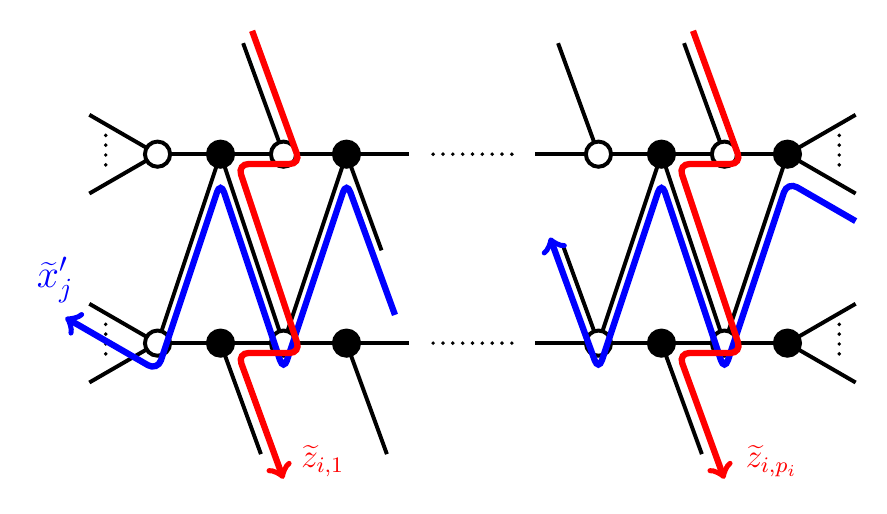
\begin{tikzpicture}
%coordinate setting
\coordinate (WW1) at (0,1.2); \coordinate (WW2) at (0,3.6);
\path (WW1) ++(0:8cm) coordinate (BB1); \path (WW2) ++(0:8cm) coordinate (BB2);
\path (BB1) ++(200:2cm) coordinate (BB0); \path (WW2) ++(20:2cm) coordinate (WW3);

\path (WW1) ++(0:0.8cm) coordinate (BB1-1); \path (WW1) ++(0:1.6cm) coordinate (WW1-1);
\path (WW1) ++(0:2.4cm) coordinate (BB1-2);
\path (WW2) ++(0:0.8cm) coordinate (BB2-1); \path (WW2) ++(0:1.6cm) coordinate (WW2-1);
\path (WW2) ++(0:2.4cm) coordinate (BB2-2);

\path (WW1) ++(0:5.6cm) coordinate (WW1-2); \path (WW1) ++(0:6.4cm) coordinate (BB1-3);
\path (WW1) ++(0:7.2cm) coordinate (WW1-3);
\path (WW2) ++(0:5.6cm) coordinate (WW2-2); \path (WW2) ++(0:6.4cm) coordinate (BB2-3);
\path (WW2) ++(0:7.2cm) coordinate (WW2-3);

\path (BB1) ++(30:1cm) coordinate (BB1e); \path (BB1) ++(330:1cm) coordinate (BB1s);
\path (WW1) ++(150:1cm) coordinate (WW1w); \path (WW1) ++(210:1cm) coordinate (WW1s);
\path (BB2) ++(30:1cm) coordinate (BB2e); \path (BB2) ++(330:1cm) coordinate (BB2s);
\path (WW2) ++(150:1cm) coordinate (WW2w); \path (WW2) ++(210:1cm) coordinate (WW2s);

\path (WW1) ++(160:0.7cm) coordinate (WW1+); \path (WW1) ++(200:0.7cm) coordinate (WW1-);
\path (WW2) ++(160:0.7cm) coordinate (WW2+); \path (WW2) ++(200:0.7cm) coordinate (WW2-);
\path (BB1) ++(20:0.7cm) coordinate (BB1+); \path (BB1) ++(340:0.7cm) coordinate (BB1-);
\path (BB2) ++(20:0.7cm) coordinate (BB2+); \path (BB2) ++(340:0.7cm) coordinate (BB2-);

%edge
\draw [line width=\edgewidth] (WW1)-- ++(0:3.2cm); \draw [line width=\edgewidth] (BB1)-- ++(180:3.2cm);
\draw [line width=\edgewidth] (WW2)-- ++(0:3.2cm); \draw [line width=\edgewidth] (BB2)-- ++(180:3.2cm);

\path (WW1) ++(0:3.5cm) coordinate (dot_start1);
\draw [line width=\edgewidth,line cap=round, dash pattern=on 0pt off 2.5\pgflinewidth] (dot_start1)-- ++(0:1.1cm);
\path (WW2) ++(0:3.5cm) coordinate (dot_start2);
\draw [line width=\edgewidth,line cap=round, dash pattern=on 0pt off 2.5\pgflinewidth] (dot_start2)-- ++(0:1.1cm);

\draw [line width=\edgewidth] (BB1)--(BB1e); \draw [line width=\edgewidth] (BB1)--(BB1s);
\draw [line width=\edgewidth] (WW1)--(WW1w); \draw [line width=\edgewidth] (WW1)--(WW1s);
\draw [line width=\edgewidth] (BB2)--(BB2e); \draw [line width=\edgewidth] (BB2)--(BB2s);
\draw [line width=\edgewidth] (WW2)--(WW2w); \draw [line width=\edgewidth] (WW2)--(WW2s);

\draw [line width=\edgewidth,line cap=round, dash pattern=on 0pt off 2.5\pgflinewidth] (WW1+)--(WW1-);
\draw [line width=\edgewidth,line cap=round, dash pattern=on 0pt off 2.5\pgflinewidth] (WW2+)--(WW2-);
\draw [line width=\edgewidth,line cap=round, dash pattern=on 0pt off 2.5\pgflinewidth] (BB1+)--(BB1-);
\draw [line width=\edgewidth,line cap=round, dash pattern=on 0pt off 2.5\pgflinewidth] (BB2+)--(BB2-);

\path (BB1-1) ++(-70:1.5cm) coordinate (BB1-1-); \draw [line width=\edgewidth] (BB1-1)--(BB1-1-);
\path (BB1-2) ++(-70:1.5cm) coordinate (BB1-2-); \draw [line width=\edgewidth] (BB1-2)--(BB1-2-);
\path (WW2-1) ++(110:1.5cm) coordinate (WW2-1-); \draw [line width=\edgewidth] (WW2-1)--(WW2-1-);
\draw [line width=\edgewidth] (BB2-1)--(WW1-1);
\draw [line width=\edgewidth] (BB2-2)-- ++(-70:1.3cm);

\path (BB1-3) ++(-70:1.5cm) coordinate (BB1-3-); \draw [line width=\edgewidth] (BB1-3)--(BB1-3-);
\path (WW2-2) ++(110:1.5cm) coordinate (WW2-2-); \draw [line width=\edgewidth] (WW2-2)--(WW2-2-);
\path (WW2-3) ++(110:1.5cm) coordinate (WW2-3-); \draw [line width=\edgewidth] (WW2-3)--(WW2-3-);
\draw [line width=\edgewidth] (BB2-3)--(WW1-3);
\draw [line width=\edgewidth] (WW1-2)-- ++(110:1.3cm);

%bypass
\draw [line width=\edgewidth] (BB2-1)--(WW1); \draw [line width=\edgewidth] (BB2-2)--(WW1-1); %\draw [line width=\edgewidth] (BB2)--(WW1-2);
\draw [line width=\edgewidth] (WW1-3)--(BB2); \draw [line width=\edgewidth] (WW1-2)--(BB2-3);

%blacknode
\draw [line width=\nodewidth, fill=black] (BB1) circle [radius=\noderad] ; \draw [line width=\nodewidth, fill=black] (BB2) circle [radius=\noderad] ;
\draw [line width=\nodewidth, fill=black] (BB1-1) circle [radius=\noderad] ; \draw [line width=\nodewidth, fill=black] (BB1-2) circle [radius=\noderad] ;
\draw [line width=\nodewidth, fill=black] (BB1-3) circle [radius=\noderad] ;
\draw [line width=\nodewidth, fill=black] (BB2-1) circle [radius=\noderad] ; \draw [line width=\nodewidth, fill=black] (BB2-2) circle [radius=\noderad] ;
\draw [line width=\nodewidth, fill=black] (BB2-3) circle [radius=\noderad] ;
%whitenode
\draw [line width=\nodewidth, fill=white] (WW1) circle [radius=\noderad] ; \draw [line width=\nodewidth, fill=white] (WW2) circle [radius=\noderad] ;
\draw [line width=\nodewidth, fill=white] (WW1-1) circle [radius=\noderad] ; \draw [line width=\nodewidth, fill=white] (WW1-2) circle [radius=\noderad] ;
\draw [line width=\nodewidth, fill=white] (WW1-3) circle [radius=\noderad] ;
\draw [line width=\nodewidth, fill=white] (WW2-1) circle [radius=\noderad] ; \draw [line width=\nodewidth, fill=white] (WW2-2) circle [radius=\noderad] ;
\draw [line width=\nodewidth, fill=white] (WW2-3) circle [radius=\noderad] ;

%zigzag path
%\path (BB2s) ++(-90:0.3cm) coordinate (BB2sz);
\path (BB2) ++(-90:0.35cm) coordinate (BB2z); \path (BB2z) ++(330:1cm) coordinate (BB2sz);
\path (WW1-3) ++(-90:0.35cm) coordinate (WW1-3z);
\path (BB2-3) ++(-90:0.35cm) coordinate (BB2-3z); \path (WW1-2) ++(-90:0.35cm) coordinate (WW1-2z);
\draw [->, rounded corners, line width=0.08cm, blue] (BB2sz)--(BB2z)--(WW1-3z)--(BB2-3z)--(WW1-2z)-- ++(110:1.8cm);

\path (WW1) ++(-90:0.35cm) coordinate (WW1z);
\path (BB2-1) ++(-90:0.35cm) coordinate (BB2-1z); \path (BB2-2) ++(-90:0.35cm) coordinate (BB2-2z);
\path (WW1-1) ++(-90:0.35cm) coordinate (WW1-1z);
\path (WW1z) ++(150:1.35cm) coordinate (WW1wz);
\draw [<-, rounded corners, line width=0.08cm, blue] (WW1wz)--(WW1z)--(BB2-1z)--(WW1-1z)--(BB2-2z)-- ++(-70:1.8cm);

\path (WW1-1) ++(-30:0.25cm) coordinate (WW1-1z); \path (BB2-1) ++(-30:0.25cm) coordinate (BB2-1z);
\path (WW2-1) ++(-30:0.25cm) coordinate (WW2-1z); \path (BB1-1) ++(-30:0.25cm) coordinate (BB1-1z);
\path (WW2-1z) ++(110:1.8cm) coordinate (WW2-1zz); \path (BB1-1z) ++(290:1.7cm) coordinate (BB1-1zz);
\draw [->, rounded corners, line width=0.08cm, red] (WW2-1zz)--(WW2-1z)--(BB2-1z)--(WW1-1z)--(BB1-1z)--(BB1-1zz);

\path (WW1-3) ++(-30:0.25cm) coordinate (WW1-3z); \path (BB2-3) ++(-30:0.25cm) coordinate (BB2-3z);
\path (WW2-3) ++(-30:0.25cm) coordinate (WW2-3z); \path (BB1-3) ++(-30:0.25cm) coordinate (BB1-3z);
\path (WW2-3z) ++(110:1.8cm) coordinate (WW2-3zz); \path (BB1-3z) ++(290:1.7cm) coordinate (BB1-3zz);
\draw [->, rounded corners, line width=0.08cm, red] (WW2-3zz)--(WW2-3z)--(BB2-3z)--(WW1-3z)--(BB1-3z)--(BB1-3zz);


\node at (-1.3,2) {\color{blue}\Large$\widetilde{x}_j^\prime$};
\node[red] at (2.1,-0.3) {\large$\widetilde{z}_{i,1}$}; \node[red] at (7.8,-0.3) {\large$\widetilde{z}_{i,p_i}$};
\end{tikzpicture}
}};
\end{tikzpicture}
\caption{The case where the projection of $\widetilde{z_i}[2m]=\widetilde{x_j}[2m+1]$ on $\Gamma$ is not contained in $X_i$.}\label{fig_observation_zigzag2}
\end{figure}

\begin{figure}[h!]\centering
\begin{tikzpicture}
\newcommand{\edgewidth}{0.05cm} %line_width_of _edges
\newcommand{\nodewidth}{0.05cm} %line_width_around_nodes
\newcommand{\noderad}{0.16} %radius_of_node

\node (original) at (0,0)
{\scalebox{0.65}{
\begin{tikzpicture}
%edge
\draw [line width=\edgewidth] (B1)--(W1); \draw [line width=\edgewidth] (B2)--(W1) ; \draw [line width=\edgewidth] (B2)--(W2) ;
\draw [line width=\edgewidth] (B1)--(B0) ; \draw [line width=\edgewidth] (W2)--(W3) ;
\draw [line width=\edgewidth] (B1)--(B1e); \draw [line width=\edgewidth] (B1)--(B1s);
\draw [line width=\edgewidth] (W1)--(W1w); \draw [line width=\edgewidth] (W1)--(W1s);
\draw [line width=\edgewidth] (B2)--(B2e); \draw [line width=\edgewidth] (B2)--(B2s);
\draw [line width=\edgewidth] (W2)--(W2w); \draw [line width=\edgewidth] (W2)--(W2s);

\draw [line width=\edgewidth,line cap=round, dash pattern=on 0pt off 2.5\pgflinewidth] (W1+)--(W1-);
\draw [line width=\edgewidth,line cap=round, dash pattern=on 0pt off 2.5\pgflinewidth] (W2+)--(W2-);
\draw [line width=\edgewidth,line cap=round, dash pattern=on 0pt off 2.5\pgflinewidth] (B1+)--(B1-);
\draw [line width=\edgewidth,line cap=round, dash pattern=on 0pt off 2.5\pgflinewidth] (B2+)--(B2-);
%blacknode
\draw [line width=\nodewidth, fill=black] (B1) circle [radius=\noderad] ; \draw [line width=\nodewidth, fill=black] (B2) circle [radius=\noderad] ;
%whitenode
\draw [line width=\nodewidth, fill=white] (W1) circle [radius=\noderad] ; \draw [line width=\nodewidth, fill=white] (W2) circle [radius=\noderad] ;

%zigzag path
\path (W1) ++(90:0.2cm) coordinate (W1z); \path (W2) ++(90:0.2cm) coordinate (W2z);
\path (B1) ++(90:0.2cm) coordinate (B1z); \path (B2) ++(90:0.2cm) coordinate (B2z);
\path (B1z) ++(225:2cm) coordinate (B0z); \path (W2z) ++(45:2cm) coordinate (W3z);

\path (B2) ++(-90:0.2cm) coordinate (B2zz); \path (B2zz) ++(330:1cm) coordinate (B2szz);
\path (W1) ++(-90:0.2cm) coordinate (W1zz); \path (W1zz) ++(150:1.5cm) coordinate (W1wzz);
\draw [->, rounded corners, line width=0.08cm, blue] (B2szz)--(B2zz)--(W1zz)--(W1wzz);
\draw [->, rounded corners, line width=0.08cm, red] (B0z)--(B1z)--(W1z)--(B2z)--(W2z)--(W3z);

\node at (0.3,4.8) {\color{red}\Large$\widetilde{z_i}$};
\node at (-1.2,2.3) {\color{blue}\Large$\widetilde{x_j}$};
\end{tikzpicture}
}};

\draw [->,line width=0.035cm] (2.6,0)--(5.2,0);
\node at (3.9,0.35) {\small(zig-1)--(zig-4)};


\node (after) at (8.9,0)
{\scalebox{0.65}{
\begin{tikzpicture}
%edge
\draw [line width=\edgewidth] (WW1)-- ++(0:3.2cm); \draw [line width=\edgewidth] (BB1)-- ++(180:3.2cm);
\draw [line width=\edgewidth] (WW2)-- ++(0:3.2cm); \draw [line width=\edgewidth] (BB2)-- ++(180:3.2cm);

\path (WW1) ++(0:3.5cm) coordinate (dot_start1);
\draw [line width=\edgewidth,line cap=round, dash pattern=on 0pt off 2.5\pgflinewidth] (dot_start1)-- ++(0:1.1cm);
\path (WW2) ++(0:3.5cm) coordinate (dot_start2);
\draw [line width=\edgewidth,line cap=round, dash pattern=on 0pt off 2.5\pgflinewidth] (dot_start2)-- ++(0:1.1cm);

\draw [line width=\edgewidth] (BB1)--(BB1e); \draw [line width=\edgewidth] (BB1)--(BB1s);
\draw [line width=\edgewidth] (WW1)--(WW1w); \draw [line width=\edgewidth] (WW1)--(WW1s);
\draw [line width=\edgewidth] (BB2)--(BB2e); \draw [line width=\edgewidth] (BB2)--(BB2s);
\draw [line width=\edgewidth] (WW2)--(WW2w); \draw [line width=\edgewidth] (WW2)--(WW2s);

\draw [line width=\edgewidth,line cap=round, dash pattern=on 0pt off 2.5\pgflinewidth] (WW1+)--(WW1-);
\draw [line width=\edgewidth,line cap=round, dash pattern=on 0pt off 2.5\pgflinewidth] (WW2+)--(WW2-);
\draw [line width=\edgewidth,line cap=round, dash pattern=on 0pt off 2.5\pgflinewidth] (BB1+)--(BB1-);
\draw [line width=\edgewidth,line cap=round, dash pattern=on 0pt off 2.5\pgflinewidth] (BB2+)--(BB2-);

\path (BB1-1) ++(-70:1.5cm) coordinate (BB1-1-); \draw [line width=\edgewidth] (BB1-1)--(BB1-1-);
\path (BB1-2) ++(-70:1.5cm) coordinate (BB1-2-); \draw [line width=\edgewidth] (BB1-2)--(BB1-2-);
\path (WW2-1) ++(110:1.5cm) coordinate (WW2-1-); \draw [line width=\edgewidth] (WW2-1)--(WW2-1-);
\draw [line width=\edgewidth] (BB2-1)--(WW1-1);
\draw [line width=\edgewidth] (BB2-2)-- ++(-70:1.3cm);

\path (BB1-3) ++(-70:1.5cm) coordinate (BB1-3-); \draw [line width=\edgewidth] (BB1-3)--(BB1-3-);
\path (WW2-2) ++(110:1.5cm) coordinate (WW2-2-); \draw [line width=\edgewidth] (WW2-2)--(WW2-2-);
\path (WW2-3) ++(110:1.5cm) coordinate (WW2-3-); \draw [line width=\edgewidth] (WW2-3)--(WW2-3-);
\draw [line width=\edgewidth] (BB2-3)--(WW1-3);
\draw [line width=\edgewidth] (WW1-2)-- ++(110:1.3cm);

%blacknode
\draw [line width=\nodewidth, fill=black] (BB1) circle [radius=\noderad] ; \draw [line width=\nodewidth, fill=black] (BB2) circle [radius=\noderad] ;
\draw [line width=\nodewidth, fill=black] (BB1-1) circle [radius=\noderad] ; \draw [line width=\nodewidth, fill=black] (BB1-2) circle [radius=\noderad] ;
\draw [line width=\nodewidth, fill=black] (BB1-3) circle [radius=\noderad] ;
\draw [line width=\nodewidth, fill=black] (BB2-1) circle [radius=\noderad] ; \draw [line width=\nodewidth, fill=black] (BB2-2) circle [radius=\noderad] ;
\draw [line width=\nodewidth, fill=black] (BB2-3) circle [radius=\noderad] ;
%whitenode
\draw [line width=\nodewidth, fill=white] (WW1) circle [radius=\noderad] ; \draw [line width=\nodewidth, fill=white] (WW2) circle [radius=\noderad] ;
\draw [line width=\nodewidth, fill=white] (WW1-1) circle [radius=\noderad] ; \draw [line width=\nodewidth, fill=white] (WW1-2) circle [radius=\noderad] ;
\draw [line width=\nodewidth, fill=white] (WW1-3) circle [radius=\noderad] ;
\draw [line width=\nodewidth, fill=white] (WW2-1) circle [radius=\noderad] ; \draw [line width=\nodewidth, fill=white] (WW2-2) circle [radius=\noderad] ;
\draw [line width=\nodewidth, fill=white] (WW2-3) circle [radius=\noderad] ;

%zigzag path
\path (BB2) ++(-110:0.28cm) coordinate (BB2z); \path (BB2z) ++(330:1.2cm) coordinate (BB2zz);
\path (WW2-3) ++(-110:0.28cm) coordinate (WW2-3z); \path (WW2-3z) ++(110:2cm) coordinate (WW2-3zz);
\draw [->, rounded corners, line width=0.08cm, blue] (BB2zz)--(BB2z)--(WW2-3z)--(WW2-3zz);

\path (WW1-1) ++(-30:0.25cm) coordinate (WW1-1z); \path (BB2-1) ++(-30:0.25cm) coordinate (BB2-1z);
\path (WW2-1) ++(-30:0.25cm) coordinate (WW2-1z); \path (BB1-1) ++(-30:0.25cm) coordinate (BB1-1z);
\path (WW2-1z) ++(110:1.8cm) coordinate (WW2-1zz); \path (BB1-1z) ++(290:1.7cm) coordinate (BB1-1zz);
\draw [->, rounded corners, line width=0.08cm, red] (WW2-1zz)--(WW2-1z)--(BB2-1z)--(WW1-1z)--(BB1-1z)--(BB1-1zz);

\path (WW1-3) ++(-30:0.25cm) coordinate (WW1-3z); \path (BB2-3) ++(-30:0.25cm) coordinate (BB2-3z);
\path (WW2-3) ++(-30:0.25cm) coordinate (WW2-3z); \path (BB1-3) ++(-30:0.25cm) coordinate (BB1-3z);
\path (WW2-3z) ++(110:1.8cm) coordinate (WW2-3zz); \path (BB1-3z) ++(290:1.7cm) coordinate (BB1-3zz);
\draw [->, rounded corners, line width=0.08cm, red] (WW2-3zz)--(WW2-3z)--(BB2-3z)--(WW1-3z)--(BB1-3z)--(BB1-3zz);

\node at (6,4.8) {\color{blue}\Large$\widetilde{x}_j^\prime$};
\node[red] at (2.1,-0.3) {\large$\widetilde{z}_{i,1}$}; \node[red] at (7.8,-0.3) {\large$\widetilde{z}_{i,p_i}$};
\end{tikzpicture}
}};
\end{tikzpicture}
\caption{The case where the projection of $\widetilde{z_i}[2m]=\widetilde{x_j}[2m+1]$ on $\Gamma$ is contained in $X_i$.}
\label{fig_observation_zigzag3}
\end{figure}

If $z_i[2m]$ is contained in $X_i$, then no bypasses are inserted.
We again consider the zigzag path $\widetilde{x}^\prime_j$ on the universal cover of $\overline{\nu}_\calX^\zig(\Gamma)$ passing through $\widetilde{x_j}[2m]$ as a zag of $\widetilde{x}^\prime_j$ (e.g., see Figure~\ref{fig_observation_zigzag3}).
Unlike in the previous case, after passing through $\widetilde{x_j}[2m]$, $\widetilde{x}^\prime_j$ goes to the edge $\big\{\widetilde{b}_i[2m+1],\widetilde{w}_{i,1}[2m+1]\big\}$.
(Here, we denote the edge whose endpoints are a~black node~$b$ and a~white node~$w$ by~$\{b,w\}$.)

If $z_i[2m+2]\in X_i$, in which case bypasses are not inserted, then $\widetilde{x}^\prime_j$ goes to the edge $\big\{\widetilde{w}_{i,1}[2m+1], \widetilde{b}_{i,1}[2m+3]\big\}$.

On the other hand, if $z_i[2m+2]\not\in X_i$, in which case we insert bypasses, then $\widetilde{x}^\prime_j$ goes to the edge $\big\{\widetilde{w}_{i,1}[2m+1], \widetilde{b}_i[2m+3]\big\}$.
In such a way, $\widetilde{x}^\prime_j$ crosses the $i$-th deformed part in the direction from the $(i+1)$-th irrelevant part to the $i$-th irrelevant part.
More precisely, if we assume that~$\widetilde{x}^\prime_j$ goes through the edge $\{\widetilde{b}_{i,s}[2m-1], \widetilde{w}_{i,s+1}[2m-1]\}$ in the $i$-th deformed part,
then $\widetilde{x}^\prime_j$ behaves as follows:
\begin{itemize}\itemsep=0pt
\item[(1)] if $z_i[2m]\in X_i$, in which case bypasses are not inserted, then $\widetilde{x}^\prime_j$ goes through the edge $\big\{\widetilde{w}_{i,s+1}[2m-1],\widetilde{b}_{i,s+1}[2m+1]\big\}$ and then $\big\{\widetilde{b}_{i,s+1}[2m+1], \widetilde{w}_{i,s+2}[2m+1]\big\}$,
\item[(2)] if $z_i[2m]\not\in X_i$, in which case we insert bypasses, then $\widetilde{x}^\prime_j$ goes through the edge $\big\{\widetilde{w}_{i,s+1}[2m-1], \widetilde{b}_{i,s}[2m+1]\big\}$ and then $\big\{\widetilde{b}_{i,s}[2m+1], \widetilde{w}_{i,s+1}[2m+1]\big\}$,
\end{itemize}
where $m=1,\dots,n$ and $s=0,\dots,p_i-1$ with $\widetilde{b}_{i,0}[-]=\widetilde{b}_i[-]$ and $\widetilde{w}_{i,p_i+1}[-]=\widetilde{w}_i[-]$.
When we consider $\widetilde{x}^\prime_j$ in the $i$-th deformed part, we encounter case (1) $|X_i|$ times and case (2) $\ell(z_i)/2-|X_i|$ times.
Since $p_i=|X_i|-1$, we see that $\widetilde{x}^\prime_j$ goes out the $i$-th deformed part from $\widetilde{w}_i[2m-1+2n]=\widetilde{w}_i[2m-1+\ell(z_i)]$,
and then it goes into the $i$-th irrelevant part.
Thus, $\widetilde{x}^\prime_j$ behaves in the same manner as the shift of $\widetilde{x}_j$ in the $i$-th irrelevant part.
For example, if we consider the type I zigzag path $z_i$ with $\ell(z_i)=8$, and the zig-deformation parameter $X_i$ with $|X_i|=3$ and $z_i[2m+4]\not\in X_i$, then the $i$-th deformed part will change as shown in Figure~\ref{fig_observation_zigzag4}.

\begin{figure}[h!]\centering
\scalebox{0.6}{
\begin{tikzpicture}
\newcommand{\edgewidth}{0.05cm} %line_width_of _edges
\newcommand{\nodewidth}{0.05cm} %line_width_around_nodes
\newcommand{\noderad}{0.17} %radius_of_node

\node at (0,0){
\begin{tikzpicture}
%%%coordinate setting
%black
\foreach \blackname/\x/\y in {3/4.5/0, 6/4.5/2, 9/4.5/4, 12/4.5/6, 15/4.5/8}
{\coordinate (B\blackname) at (\x,\y);}
%white
\foreach \whitename/\x/\y in {1/0/0, 4/0/2, 7/0/4, 10/0/6, 13/0/8}
{\coordinate (W\whitename) at (\x,\y);}

%%%edges
\foreach \t/\h in {1/3,4/6,7/9,10/12,13/15}{\draw [line width=\edgewidth] (W\t)--(B\h); } %horizontal line
\foreach \t/\h in {1/6,4/9,7/12,10/15}{\draw [line width=\edgewidth] (W\t)--(B\h); }
\foreach \t in {3}{\draw [line width=\edgewidth] (B\t)-- ++(210:1.2cm); }
\foreach \t in {13}{\draw [line width=\edgewidth] (W\t)-- ++(30:1.2cm); }

%boundary_edges
\foreach \t in {1,4,7,10,13}{\draw [line width=\edgewidth] (W\t)-- ++(150:1cm); \draw [line width=\edgewidth] (W\t)-- ++(210:1cm); }
\foreach \t in {1,4,7,10,13}{\path (W\t) ++ (165:0.7cm) coordinate (W\t+); \draw [line width=\edgewidth,line cap=round, dash pattern=on 0pt off 2.5\pgflinewidth] (W\t+)-- ++(-90:0.38cm);}
\foreach \t in {3,6,9,12,15}{\draw [line width=\edgewidth] (B\t)-- ++(30:1cm); \draw [line width=\edgewidth] (B\t)-- ++(-30:1cm); }
\foreach \t in {3,6,9,12,15}{\path (B\t) ++ (15:0.7cm) coordinate (B\t+); \draw [line width=\edgewidth,line cap=round, dash pattern=on 0pt off 2.5\pgflinewidth] (B\t+)-- ++(-90:0.38cm);}

%%%nodes
%blacknode
\foreach \n in {3,6,9,12,15} {\draw [line width=\nodewidth, fill=black] (B\n) circle [radius=\noderad];}
%whitenode
\foreach \n in {1,4,7,10,13} {\draw [line width=\nodewidth, fill=white] (W\n) circle [radius=\noderad];}

%zigzag
\path (B6) ++(-90:0.2cm) coordinate (B6_z); \path (W1) ++(-90:0.2cm) coordinate (W1_z);
\path (B6_z) ++(-30:1.2cm) coordinate (B6_zz); \path (W1_z) ++(150:1.2cm) coordinate (W1_zz);
\draw [->, rounded corners, line width=0.09cm, blue] (B6_zz)--(B6_z)--(W1_z)--(W1_zz);

\path (W13) ++(-90:0.2cm) coordinate (W13_z); \path (W13_z) ++(150:1.2cm) coordinate (W13_zz+);
\path (W13_z) ++(30:1.2cm) coordinate (W13_zz-);
\draw [->, rounded corners, line width=0.09cm, blue] (W13_zz-)--(W13_z)--(W13_zz+);

%node
\path (W1_zz) ++(180:0.3cm) node[blue] {\large $\widetilde{x}_j$};
\path (W13_zz+) ++(180:0.6cm) node[blue] {\large $\widetilde{x}_j(1)$};

\node[red] at (2.25,-0.3) {$\widetilde{z}_i[2m-1]$}; \node[red] at (2.25,1.3) {$\widetilde{z}_i[2m]$};
\node[red] at (2.25,2.3) {$\widetilde{z}_i[2m+1]$}; \node[red] at (2.25,8.3) {$\widetilde{z}_i[2m+7]$};
\path (W1) ++(-90:0.86cm) node {$\widetilde{w}_i[2m-1]$}; \path (W13) ++(90:0.86cm) node {$\widetilde{w}_i[2m+7]$};
\path (B3) ++(-90:0.86cm) node {$\widetilde{b}_i[2m-1]$}; \path (B15) ++(90:0.86cm) node {$\widetilde{b}_i[2m+7]$};
\end{tikzpicture}};

\draw [->,line width=0.05cm] (4.5,0)--(9.7,0);
\node at (7.1,0.5) {\LARGE(zig-1)--(zig-4)};

\node at (15,0){
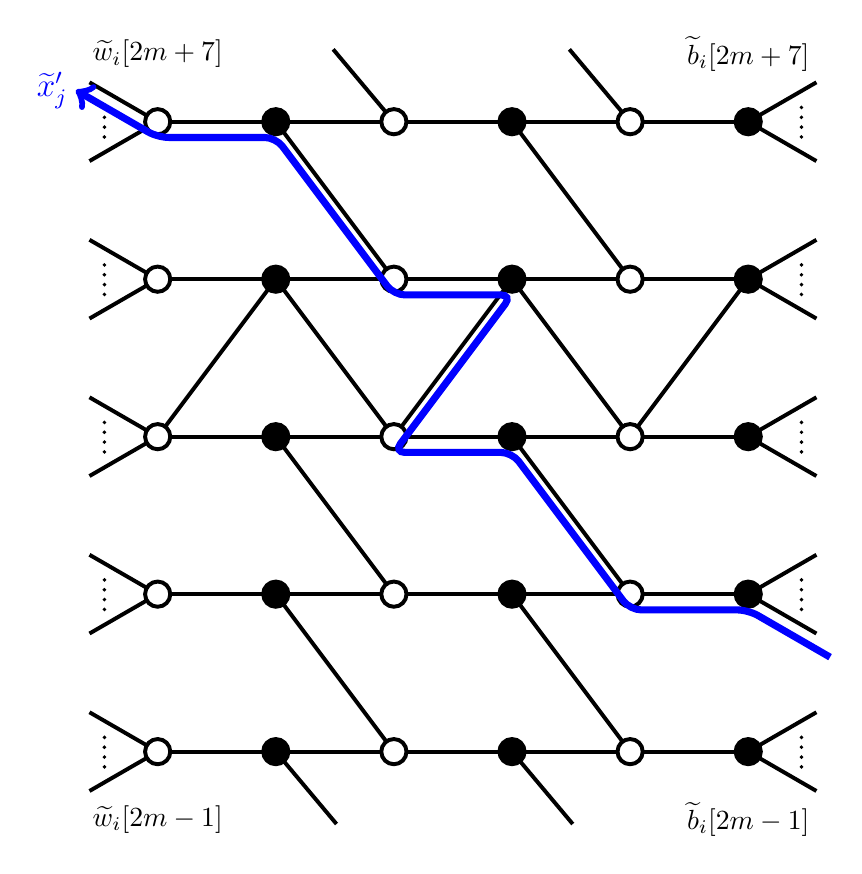
\begin{tikzpicture}
%%%coordinate setting
%black
\foreach \blackname/\x/\y in {1/1.5/0, 2/4.5/0, 3/7.5/0, 4/1.5/2, 5/4.5/2, 6/7.5/2, 7/1.5/4, 8/4.5/4, 9/7.5/4, 10/1.5/6, 11/4.5/6, 12/7.5/6, 13/1.5/8, 14/4.5/8, 15/7.5/8}
{\coordinate (B\blackname) at (\x,\y);}
%white
\foreach \whitename/\x/\y in {1/0/0, 2/3/0, 3/6/0, 4/0/2, 5/3/2, 6/6/2, 7/0/4, 8/3/4, 9/6/4, 10/0/6, 11/3/6, 12/6/6, 13/0/8, 14/3/8, 15/6/8}
{\coordinate (W\whitename) at (\x,\y);}

%%%edges
\foreach \t/\h in {1/3,4/6,7/9,10/12,13/15}{\draw [line width=\edgewidth] (W\t)--(B\h); } %horizontal line
\foreach \t/\h in {2/4,3/5,5/7,6/8,8/10,9/11,11/13,12/14}{\draw [line width=\edgewidth] (W\t)--(B\h); }
\foreach \t/\h in {7/10,8/11,9/12}{\draw [line width=\edgewidth] (W\t)--(B\h); } %bypass

\foreach \t in {1,2}{\draw [line width=\edgewidth] (B\t)-- ++(-50:1.2cm); }
\foreach \t in {14,15}{\draw [line width=\edgewidth] (W\t)-- ++(130:1.2cm); }

%boundary_edges
\foreach \t in {1,4,7,10,13}{\draw [line width=\edgewidth] (W\t)-- ++(150:1cm); \draw [line width=\edgewidth] (W\t)-- ++(210:1cm); }
\foreach \t in {1,4,7,10,13}{\path (W\t) ++ (165:0.7cm) coordinate (W\t+); \draw [line width=\edgewidth,line cap=round, dash pattern=on 0pt off 2.5\pgflinewidth] (W\t+)-- ++(-90:0.38cm);}
\foreach \t in {3,6,9,12,15}{\draw [line width=\edgewidth] (B\t)-- ++(30:1cm); \draw [line width=\edgewidth] (B\t)-- ++(-30:1cm); }
\foreach \t in {3,6,9,12,15}{\path (B\t) ++ (15:0.7cm) coordinate (B\t+); \draw [line width=\edgewidth,line cap=round, dash pattern=on 0pt off 2.5\pgflinewidth] (B\t+)-- ++(-90:0.38cm);}

%%%nodes
%blacknode
\foreach \n in {1,2,3,4,5,6,7,8,9,10,11,12,13,14,15} {\draw [line width=\nodewidth, fill=black] (B\n) circle [radius=\noderad];}
%whitenode
\foreach \n in {1,2,3,4,5,6,7,8,9,10,11,12,13,14,15} {\draw [line width=\nodewidth, fill=white] (W\n) circle [radius=\noderad];}

%zigzag
\foreach \t in {6,8,11,13}{\path (B\t) ++(-90:0.2cm) coordinate (B\t_z); }
\foreach \t in {6,8,11,13}{\path (W\t) ++(-90:0.2cm) coordinate (W\t_z); }
\path (B6_z) ++(-30:1.2cm) coordinate (B6_zz); \path (W13_z) ++(150:1.2cm) coordinate (W13_zz);
\draw [->, rounded corners, line width=0.09cm, blue] (B6_zz)--(B6_z)--(W6_z)--(B8_z)--(W8_z)--(B11_z)--(W11_z)--(B13_z)--(W13_z)--(W13_zz);

%node
\path (W13_zz) ++(180:0.3cm) node[blue] {\large $\widetilde{x}_j^\prime$};

\path (W1) ++(-90:0.86cm) node {$\widetilde{w}_i[2m-1]$}; \path (W13) ++(90:0.86cm) node {$\widetilde{w}_i[2m+7]$};
\path (B3) ++(-90:0.86cm) node {$\widetilde{b}_i[2m-1]$}; \path (B15) ++(90:0.86cm) node {$\widetilde{b}_i[2m+7]$};
\end{tikzpicture}};

\end{tikzpicture}
}
\caption{An example of the behavior of $\widetilde{x}^\prime_j$ in the $i$-th deformed part.}
\label{fig_observation_zigzag4}
\end{figure}
\end{observation}

\subsection{Properties of zigzag paths on deformed dimer models}\label{subsec_property_zigzag}

In this subsection, we study the slopes of zigzag paths on deformed dimer models.
In particular, we can describe them in terms of zigzag paths of the original dimer model, and this description plays a crucial role when discussing the relationship with the combinatorial mutations of the associated polygons.

\begin{Proposition}\label{deform_vector}
The path $z_{i,j}$ given in {\rm(zig-3)} of Definition~{\rm \ref{def_deformation_zig}} $($resp.\ {\rm(zag-3)} of Definition~{\rm \ref{def_deformation_zag})} is a type I zigzag path $z_{i,j}$ of $\nu^\zig_\calX(\Gamma)$ $($resp.~$\nu^\zag_\calY(\Gamma)$$)$ with $\ell(z_{i,j})=\ell(z_i)$.
Moreover, $z_{i,j}$ does not have any self-intersections on the universal cover, and satisfies $[z_{i,j}]=-[z_i]=-v$, and hence it is not homologically trivial.
\end{Proposition}

\begin{proof}
We consider the case of $\nu^\zig_\calX(\Gamma)$. The case of $\nu^\zag_\calY(\Gamma)$ is similar.

First, $z_{i,j}$ is a zigzag path of $\overline{\nu}^\zig_\calX(\Gamma)$ by definition.
We see that zigzag paths of $\overline{\nu}^\zig_\calX(\Gamma)$ intersecting with $\widetilde{z}_{i,j}$ take either the form of $\widetilde{y}_k^\prime$ given in Observation~\ref{obs_deformed_part2} or $\widetilde{x}_j^\prime$ given in Observation~\ref{obs_deformed_part3}.
In particular, these intersect with $\widetilde{z}_{i,j}$ precisely once in each deformed part, and
$\widetilde{y}_k^\prime$ crosses the $i$-th deformed part in the direction from the $i$-th irrelevant part to the $(i+1)$-th irrelevant part, and $\widetilde{x}_j^\prime$ crosses the $i$-th deformed part in the direction from the $(i+1)$-th irrelevant part to the $i$-th irrelevant part for all $i$.
Since other zigzag paths do not intersect with $\widetilde{z}_{i,j}$, we see that $z_{i,j}$ is a type I zigzag path of $\overline{\nu}^\zig_\calX(\Gamma)$.
Also, $\widetilde{z}_{i,j}$ does not have any self-intersections by definition.
By these properties, the edges constituting $z_{i,j}$ are not removed by the operation (zig-5).
In addition, since $z_{i,j}$ contains no $2$-valent nodes, the operation (join) does not affect $z_{i,j}$.
Therefore, we see that $z_{i,j}$ is a type I zigzag path of $\nu^\zig_\calX(\Gamma)$, and the remaining assertions follow from the definition of $z_{i,j}$.
\end{proof}

\begin{Proposition}\label{zigzag_afterdeform1}
The paths $y_1,\dots, y_t$ $($resp.\ the paths $x_1,\dots, x_s)$ are zigzag paths of $\Gamma$ intersecting with a chosen type~I zigzag path~$z$
at some zigs $($resp.\ zags$)$ of $z$. We have the following.
\begin{itemize}\itemsep=0pt
\item[\rm (1)] For any zigzag path $y_k$ of $\Gamma$, there exists a unique zigzag path $y_k^\prime$ of $\nu^\zig_\calX(\Gamma)$ without self-intersections
on the universal cover and satisfying $[y_k]=[y_k^\prime]$ where $k=1,\dots,t$.
\item[\rm (2)] For any zigzag path $x_j$ of $\Gamma$, there exists a unique zigzag path $x_j^\prime$ of $\nu^\zag_\calY(\Gamma)$ without self-intersections
on the universal cover and satisfying $[x_j]=[x_j^\prime]$ where $j=1,\dots,s$.
\end{itemize}
\end{Proposition}

\begin{proof}We consider the case of $\nu^\zig_\calX(\Gamma)$. The case of $\nu^\zag_\calY(\Gamma)$ is similar.

We use the same notation used in Observation~\ref{obs_deformed_part2}.
In particular, we consider the zigzag path~$\widetilde{y}^\prime_k$ of~$\widetilde{\Gamma}^\prime$ which coincides with $\widetilde{y}_k$ in all irrelevant parts, and behaves as depicted on the right-hand side of Figure~\ref{fig_observation_zigzag1} in each deformed part,
and therefore does not have any self-intersections.
Since bypasses inserted in the operation~(zig-4) do not affect the behavior of $\widetilde{y}^\prime_k$, we can extend $\widetilde{y}^\prime_k$ to a zigzag path of the universal cover of $\overline{\nu}^\zig_\calX(\Gamma)$.
By projecting $\widetilde{y}^\prime_k$ onto~$\overline{\nu}^\zig_\calX(\Gamma)$, we have the zigzag path $y_k^\prime$ of $\overline{\nu}^\zig_\calX(\Gamma)$.
By the construction given in Observation~\ref{obs_deformed_part2}, we see that $[y_k]=[y_k^\prime]$.
Since~$\widetilde{y}^\prime_k$ coincides with $\widetilde{y}_k$ in all irrelevant parts and $\Gamma$ is consistent, it does not behave pathologically in irrelevant parts as it infringes on the consistency condition.
Furthermore, $\widetilde{y}^\prime_k$ intersects with zigzag paths of the forms $\widetilde{z}_{i,j}$ and $\widetilde{x}^\prime_j$ (see Observation~\ref{obs_deformed_part3}) in some deformed parts, but they do not intersect with each other in the same direction more than once.
Therefore, the edges constituting~$y_k^\prime$ are not removed by the operation~(zig-5), and hence~$y_k^\prime$ is not changed by~(zig-5).
In addition, the operation (join) does not change the slopes.
Thus, we naturally extend this zigzag path $y_k^\prime$ as the path of $\nu^\zig_\calX(\Gamma)$, which is determined uniquely and satisfies $[y_k]=[y_k^\prime]$ by construction.
\end{proof}

By the proof of Propositions~\ref{deform_vector} and \ref{zigzag_afterdeform1}, the zigzag paths $\widetilde{z}_{i,j}$
and $\widetilde{y}^\prime_k$ do not have any self-intersections,
and do not intersect with other zigzag paths in the same direction more than once.
Furthermore, the intersections between $\widetilde{x}^\prime_j$ and $\widetilde{z}_{i,j}$ or $\widetilde{y}^\prime_k$ are not bypasses
(see Observations~\ref{obs_deformed_part2} and \ref{obs_deformed_part3}). This proves the following lemma.

\begin{Lemma}\label{bypass_removable}
We have the following.
\begin{itemize}\itemsep=0pt
\item[\rm (1)] The edges removed by the operation {\rm(zig-5)} are a part of the bypasses added in {\rm(zig-4)} or edges appearing in some irrelevant parts that are intersections between pairs of zigzag paths $x_1,\dots,x_s$.
\item[\rm (2)] The edges removed by the operation {\rm(zag-5)} are a part of the bypasses added in {\rm(zag-4)} or edges appearing in some irrelevant parts that are intersections between pairs of zigzag paths $y_1,\dots,y_t$.
\end{itemize}
\end{Lemma}

Before showing the next proposition, we introduce some notation.

\begin{setting}\label{setting_PMs_z}
Let $z$ be a zigzag path on a consistent dimer model $\Gamma$.
We recall that corner perfect matchings are ordered in the anti-clockwise direction along the vertices of~$\Delta_\Gamma$ (see Section~\ref{subsection_PM}).
Let~$\sfP$,~$\sfP^\prime$ be adjacent corner perfect matchings on~$\Gamma$ such that the difference of~$\sfP$ and~$\sfP^\prime$ contains~$z$ (see Proposition~\ref{zigzag_sidepolygon}).
We assume that~$\sfP$,~$\sfP^\prime$ are ordered with this order, in which case $\sfP\cap z=\Zig(z)$ and $\sfP^\prime\cap z=\Zag(z)$.
Then, we set $\sfP_z\coloneqq \sfP$ and $\sfP^\prime_z\coloneqq (\sfP{\setminus}\Zig(z))\cup\Zag(z)$.
By Proposition~\ref{char_bound}, $\sfP_z$, $\sfP^\prime_z$ are boundary perfect matchings corresponding to certain lattice points on the edge of $\Delta_\Gamma$ whose outer normal vector is~$[z]$,
and we see that the difference of~$\sfP_z$ and~$\sfP^\prime_z$, namely $\sfP_z\cup\sfP^\prime_z{\setminus}\sfP_z\cap\sfP^\prime_z$, forms~$z$.
Thus, by this construction, $h(\sfP^\prime_z,\sfP_z)\in\ZZ^2$ is a primitive lattice element with $\langle[z],h(\sfP^\prime_z,\sfP_z)\rangle=0$.
\end{setting}

\begin{Proposition}\label{zigzag_afterdeform2}
Let $h(\sfP^\prime_z,\sfP_z)$ be a primitive lattice element as above.
We have the following.
\begin{itemize}\itemsep=0pt
\item[\rm (1)] For any zigzag path $x_j$ of $\Gamma$,
there exists a unique zigzag path $x_j^\prime$ of $\nu^\zig_\calX(\Gamma)$ such that for every $j=1,\dots,s$
\begin{displaymath}
[x^{\prime}_j]=[x_j]+\langle [x_j],h(\sfP_z^\prime,\sfP_z)\rangle[z].
\end{displaymath}
\item[\rm (2)] For any zigzag path $y_k$ of $\Gamma$, there exists a unique zigzag path $y_k^\prime$ of $\nu^\zag_\calY(\Gamma)$ such that for every $k=1,\dots,t$
\begin{displaymath}
[y^{\prime}_k]=[y_k]+\langle [y_k],h(\sfP_z^\prime,\sfP_z)\rangle[z].
\end{displaymath}
\end{itemize}
\end{Proposition}

\begin{proof}We consider the case of $\nu^\zig_\calX(\Gamma)$. The case of $\nu^\zag_\calY(\Gamma)$ is similar.

We recall that $|x_j\cap z|=|x_j\cap z_i|$ for all $i=1,\dots,r$, and that this number is denoted by $m_j$ (see Definition~\ref{def_deformation_data}).
We first show that
\begin{equation}\label{desired_eq1}
m_j=\langle [x_j],h(\sfP_z^\prime,\sfP_z)\rangle
\end{equation}
for $j=1,\dots,s$. Let $p_{x_j}$ be the path of the quiver $Q_\Gamma$ going along the left side of~$x_j$ (see Observation~\ref{height_zigzag}).
In particular, considering $p_{x_j}$ as an element in $\rmH_1(\TT)$, we have $[p_{x_j}]=[x_j]$.
By our assumption, the intersections~$x_j\cap z$ are contained in $\Zag(z)=\sfP^\prime\cap z$.
Thus, $p_{x_j}$ crosses~$z$ at a~zig of~$z$.
Since $\sfP\cap z=\Zig(z)$, every time $p_{x_j}$ crosses $z$, the height function $\sfh_{\sfP^\prime,\sfP}$ increases by~$1$.
Since $m_j=|x_j\cap z|$, we have the equation~(\ref{desired_eq1}).

Then, we show that for each $x_j$ where $j=1,\dots,s$, there exists a zigzag path $x^{\prime}_j$ on $\overline{\nu}_\calX^\zig(\Gamma)=\overline{\nu}_\calX^\zig(\Gamma,\{z_1,\dots,z_r\})$ such that
\begin{equation}\label{desired_eq2}
[x^{\prime}_j]=[x_j]+m_j[z].
\end{equation}
We divide $x_j$ into sub-zigzag paths $x_j^{(1)},\dots,x_j^{(m_j)}$. By definition, $x_j^{(1)}$ intersects with $z_r$ at a~zag of~$z_r$.
We denote this zag by $z_r[2m]\coloneqq x_j^{(1)}\cap z_r$, in which case the white (resp.\ black) node that is the end point of $z_r[2m]$ is denoted by $w_r[2m-1]$ (resp.~$b_r[2m+1]$).
By considering the universal cover $\widetilde{\Gamma}$, we naturally define $\widetilde{x}_j$, $\widetilde{x}_j^{(1)}$, $\widetilde{z}_r$, $\widetilde{z}_r[2m]$, $\widetilde{w}_r[2m-1]$, $\widetilde{b}_r[2m+1]$, etc.
Also, we assume that~$\widetilde{z}_r$ is contained in the~$(r,0)$-th deformed part.
Then, $\widetilde{x}_j$ crosses the $(r,0)$-th deformed part in the direction from the $(r+1,0)$-th irrelevant part to the $(r,0)$-th irrelevant part,
in which case the entrance of the $(r,0)$-th deformed part is $\widetilde{b}_r[2m+1]$ and the exit is $\widetilde{w}_r[2m-1]$.

In what follows, we use the same notation used in Observation~\ref{obs_deformed_part3}.
In particular, we pay attention to the zigzag path $\widetilde{x}_j^\prime$ of the universal cover $\overline{\nu}_\calX^\zig(\Gamma)^\sim$ of $\overline{\nu}_\calX^\zig(\Gamma)$, which behaves as follows:
\begin{itemize}\itemsep=0pt
\item[$(A_r)$] If $z_r[2m]\not\in X_r$, then $\widetilde{x}_j^\prime$ goes into the $(r,0)$-th deformed part of $\overline{\nu}_\calX^\zig(\Gamma)^\sim$ from $\widetilde{b}_r[2m+1]$ and goes out from $\widetilde{w}_r[2m-1]$ (see also Figure~\ref{fig_observation_zigzag2}).
After crossing the $(r,0)$-th deformed part, it goes into the $(r,0)$-th irrelevant part, and it behaves in the same manner as $\widetilde{x}_j$ in that part.
\item[$(B_r)$] If $z_r[2m]\in X_r$, then $\widetilde{x}_j^\prime$ goes into the $(r,0)$-th deformed part of $\overline{\nu}_\calX^\zig(\Gamma)^\sim$ from $\widetilde{b}_r[2m+1]$ and goes out from $\widetilde{w}_r[2m-1+2n]=\widetilde{w}_r[2m-1+\ell(z)]$ (see also Figures~\ref{fig_observation_zigzag3} and \ref{fig_observation_zigzag4}).
After crossing the $(r,0)$-th deformed part, it goes into the $(r,0)$-th irrelevant part, and it behaves in the same manner as the shift of $\widetilde{x}_j$, which we denote as $\widetilde{x}_j(1)$, in that part.
\end{itemize}
Then, $\widetilde{x}_j^\prime$ goes into the $(r-1,0)$-th deformed part of $\overline{\nu}_\calX^\zig(\Gamma)^\sim$.
We let $\widetilde{z}_{r-1}[2m^\prime]\coloneqq \widetilde{x}_j\cap \widetilde{z}_{r-1}$ and $\widetilde{z}_{r-1}[2m^{\prime\prime}]\coloneqq \widetilde{x}_j(1)\cap \widetilde{z}_{r-1}$.
We note that on the dimer model $\Gamma$ we have $z_{r-1}[2m^\prime]=z_{r-1}[2m^{\prime\prime}]=x_j^{(1)}\cap z_{r-1}$ by definition.
\begin{itemize}\itemsep=0pt
\item If $z_r[2m]\in X_r$ in the above argument, then $z_{r-1}[2m^\prime]\not\in X_{r-1}$ by the definition of~$X_r$ and~$X_{r-1}$.
(Furthermore, $x_j^{(1)}\cap z_i\not\in X_i$ for any $i\neq r$.)
In this case, $\widetilde{x}_j^\prime$ crosses the $(r-1,0)$-th deformed part of $\overline{\nu}_\calX^\zig(\Gamma)^\sim$ in the same manner as $(A_r)$ above.
Then, it behaves in the same manner as $\widetilde{x}_j(1)$ in the $(r-1,0)$-th irrelevant part.
\item Let $z_r[2m]\not\in X_r$ in the above argument.
\begin{itemize}\itemsep=0pt
\item If $z_{r-1}[2m^\prime]\not\in X_{r-1}$, then $\widetilde{x}_j^\prime$ crosses the $(r-1,0)$-th deformed part of $\overline{\nu}_\calX^\zig(\Gamma)^\sim$ in the same way as~$(A_r)$.
Then, it behaves in the same manner as $\widetilde{x}_j$ in the $(r-1,0)$-th irrelevant part.
\item If $z_{r-1}[2m^\prime]\in X_{r-1}$, then $\widetilde{x}_j^\prime$ crosses the $(r-1,0)$-th deformed part of $\overline{\nu}_\calX^\zig(\Gamma)^\sim$ in the same way as~$(B_r)$.
Then, it behaves in the same manner as $\widetilde{x}_j(1)$ in the~$(r-1,0)$-th irrelevant part.
\end{itemize}
\end{itemize}
Repeating these inductive arguments, we see that $\widetilde{x}^\prime_j$ crosses the $(i,0)$-th deformed part of $\overline{\nu}_\calX^\zig(\Gamma)^\sim$ for $i=r,r-1,\dots,1$ in this order, and goes into the $(1,0)$-th irrelevant part.
In any case, $\widetilde{x}^\prime_j$ behaves in the same manner as $\widetilde{x}_j(1)$ in this irrelevant part.

Then, $\widetilde{x}^\prime_j$ goes into the $(r,-1)$-th deformed part, in which case we consider the sub-zigzag path $x_j^{(2)}$ of~$\Gamma$
and the intersection between $\widetilde{z}_r(-1)$ and $\widetilde{x}_j^{(2)}$ on~$\widetilde{\Gamma}$.
By the same arguments as above, we see that $\widetilde{x}^\prime_j$ crosses the $(i,-1)$-th deformed part of $\overline{\nu}_\calX^\zig(\Gamma)^\sim$ for $i=r,r-1,\dots,1$ in this order.
After that, it goes into $(1,-1)$-th irrelevant part and behaves in the same manner as~$\widetilde{x}_j(2)$ in this irrelevant part.

Repeating these arguments, we finally see that $\widetilde{x}^\prime_j$ crosses the $(i,-m_j+1)$-th deformed part of $\overline{\nu}_\calX^\zig(\Gamma)^\sim$ for $i=r,r-1,\dots,1$ in this order,
and behaves in the same manner as $\widetilde{x}_j(m_j)$ in the $(1,-m_j+1)$-th irrelevant part.
Then, $\widetilde{x}^\prime_j$ goes into the $(r,-m_j)$-th deformed part of $\overline{\nu}_\calX^\zig(\Gamma)^\sim$, in which case
we denote the black node that is the entrance of this deformed part by~$B$.
Since $m_j=|x_j\cap z_i|$, the projection of $\widetilde{x}_j\cap \widetilde{z}_i(-m_j)$ on~$\Gamma$ coincides with $z_i[2m]$, which is the starting edge of our arguments.
Thus, $B$ coincides with $\widetilde{b}_r[2m+1]$ if they are projected onto $\overline{\nu}_\calX^\zig(\Gamma)$,
which means we can follow all edges of the zigzag path $x^\prime_j$ of $\overline{\nu}_\calX^\zig(\Gamma)$.
By these arguments, we see that the slope of~$\widetilde{x}^\prime_j$ changes $[z]$ in each deformed part, and thus we have $[x^{\prime}_j]=[x_j]+m_j[z]$.

Finally, we apply the operations (zig-5) and (join) to $\overline{\nu}_\calX^\zig(\Gamma)$.
Then, we obtain the deformed dimer model $\nu_\calX^\zig(\Gamma)$ and the zigzag path on it having the same slope as $\widetilde{x}^\prime_j$.
This zigzag path is determined uniquely by the construction, and we use the same notation for this zigzag path by abuse of the notation.
Since (zig-5) and (join) do not change the slopes of zigzag paths, we have~(\ref{desired_eq2}).
\end{proof}

Since the slopes of zigzag paths $\nu^\zig_\calX(\Gamma)$ and $\nu^\zag_\calY(\Gamma$) do not depend on
the choice of $X_1,\dots,X_r$ (resp.\ $Y_1,\dots,Y_r$) by Propositions~\ref{deform_vector}, \ref{zigzag_afterdeform1} and \ref{zigzag_afterdeform2},
we obtain the proposition below.
However, we remark that the deformed dimer model depends on the choice of zig-deformation parameters; thus $\nu^\zig_\calX(\Gamma,\{z_1,\dots,z_r\})\not\cong\nu^\zig_{\calX^\prime}(\Gamma,\{z_1,\dots,z_r\})$ in general (the zag version is similar).

\begin{Proposition}\label{other_weight_PMpolygon}
For zig-deformation parameter $\calX^\prime\coloneqq\{X_1^\prime,\dots,X_r^\prime\}$ and
zag-deformation parameter $\calY^\prime\coloneqq\{Y_1^\prime,\dots,Y_r^\prime\}$ different from $\calX$ and $\calY$, we have
\begin{displaymath}
\Delta_{\nu^\zig_\calX(\Gamma,\{z_1,\dots,z_r\})}=\Delta_{\nu^\zig_{\calX^\prime}(\Gamma,\{z_1,\dots,z_r\})}\qquad\text{and}\qquad \Delta_{\nu^\zag_\calY(\Gamma,\{z_1,\dots,z_r\})}=\Delta_{\nu^\zag_{\calY^\prime}(\Gamma,\{z_1,\dots,z_r\})}.
\end{displaymath}
\end{Proposition}
